\documentclass[11pt, oneside]{scrbook}

\usepackage[linear, secthm]{handout}
\usepackage{scrhack}
\usepackage[normalem]{ulem}


%% New Commands %%
\newcommand{\lecture}[1]{\noindent\rule[0.35em]{0.4\textwidth}{1pt} \hfill \fbox{\large\textsc{Lecture #1}} \hfill \rule[0.35em]{0.4\textwidth}{1pt}\addcontentsline{toc}{chapter}{\protect\numberline{}Lecture #1}}

% Ch01 - Axiomatic Set Theory %
\DeclareMathOperator{\id}{id}
\DeclareMathOperator{\lxor}{\veebar}
\DeclareMathOperator{\lnand}{\uparrow}
\usepackage{stmaryrd}
\DeclareMathOperator{\contra}{\lightning}
% \DeclareMathOperator{\im}{im} % already defined as \img
\newcommand{\0}{\emptyset}
\DeclareMathOperator{\preimg}{preim}
\DeclareMathAlphabet{\euscr}{U}{eus}{m}{n}
\DeclareMathOperator{\powerset}{\euscr{P}}
\DeclareMathOperator{\setIso}{\cong_{\text{set}}}
\usetikzlibrary{cd}
\renewcommand{\nsim}{\not\sim}
\newcommand{\into}{\hookrightarrow}

% Ch02 - Topological Spaces %
\renewcommand{\O}{\mathcal{O}}
\newcommand{\Ostd}{\mathcal{O}_{\text{std.}}}
\newcommand{\Oq}[1]{\mathcal{O}_{\faktor{#1}{\sim}}}
\DeclareMathOperator{\topIso}{\cong_{\text{top.}}}
\DeclareMathOperator{\supp}{supp}
\DeclareMathOperator{\dcup}{\dot{\cup}}
\DeclareMathOperator{\grpIso}{\cong_{\text{grp}}}

\makeatletter
\def\input@path{{Ch01 - Axiomatic Set Theory/}{Ch02 - Topological Spaces/}{Ch03 - Topological Manifolds and Bundles/}}
\makeatother


\title{
    \Huge Lecture Notes
}

\subtitle{
    \huge Geometric Anatomy of Theoretical Physics \\[10pt]
    \LARGE\normalfont\sffamily Dr. Fredric P Schuller\thanks{YouTube \href{https://youtube.com/playlist?list=PLPH7f_7ZlzxTi6kS4vCmv4ZKm9u8g5yic&si=Uy5ciENkuiTlvx6X}{playlist}}
}

\author{
\Large Piyush Kumar Singh \thanks{{\href{https://iampiyushkrsingh.github.io}{iamPiyushKrSingh.github.io}}}
}

\date{
    \large December 2024
}

%% Image Path %%
\graphicspath{{images/}}
\svgpath{{images/}}

%% TOC Setup %%
\setcounter{tocdepth}{3}
\setcounter{secnumdepth}{3}

\changemaincolor{Emerald}
\changesecondcolor{Periwinkle}

\hypersetup{
    pdftitle={Geometric Anatomy of Theoretical Physics},
    pdfauthor={Piyush Kumar Singh, Fredric Schuller},
    pdfkeywords={Quantum Mechanics, physics, qm, topology, geometry, notes, differentialbe manifold, theoretical physics, geometric anatomy},
    linktocpage=true
}

\begin{document}
\frontmatter
\begin{titlepage}
	\let\newpage\relax
	\singhtitle
\end{titlepage}

\chapter{Structure of this Course}
\noindent In theoretical physics we mainly deal with three big part of mathematics, namely, `Analysis', `Algebra' and `Geometry'. And at the mutual intersection of these three, we have different branches of physics like `Quantum Mechanics', `General Relativity', `Statistical Mechanics', etc. see \cref{fig:structure}.

\begin{figure}[H]
	\centering
	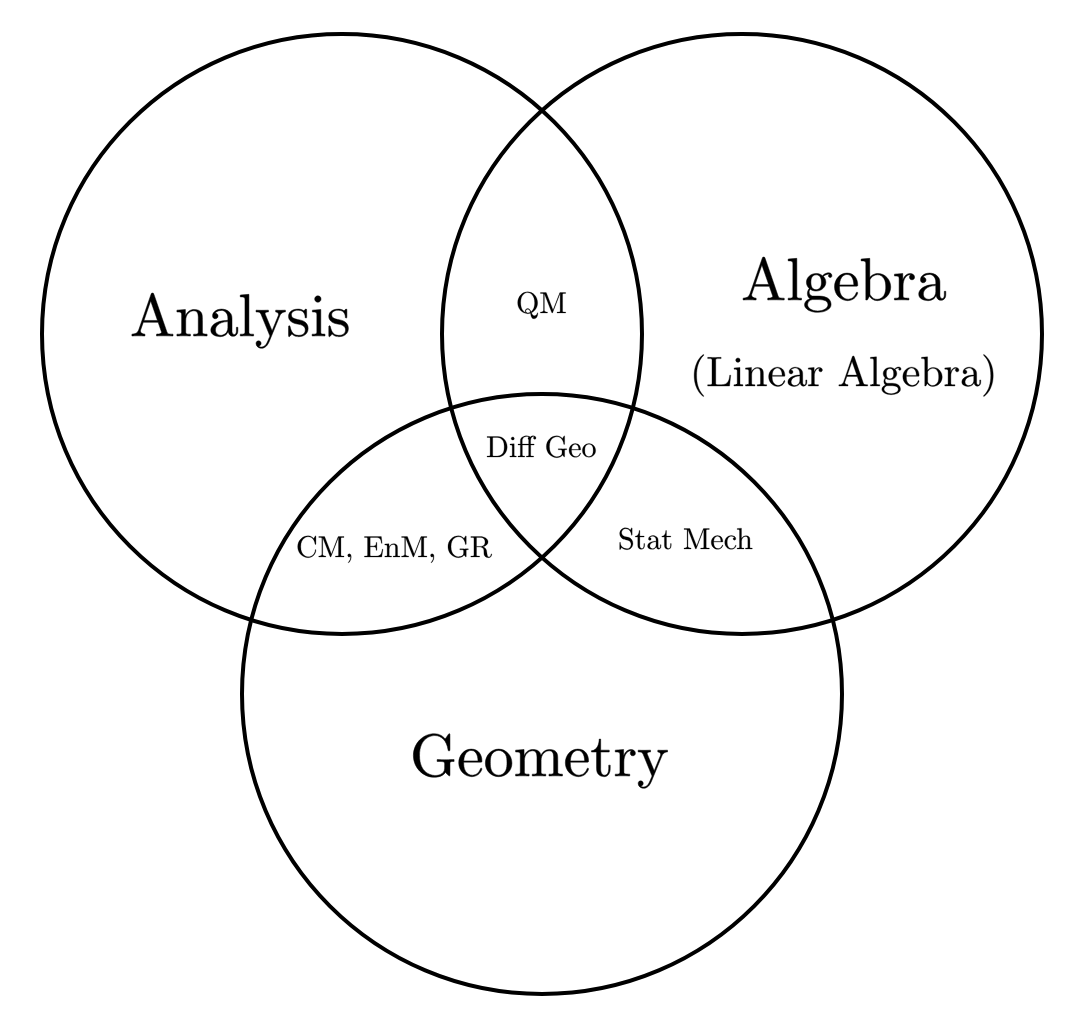
\includegraphics[width=0.4\textwidth]{lec01-math_struct.png}
	\caption{Structure of Theoretical Physics}
	\label{fig:structure}
\end{figure}\noindent
This course mainly focuses on differential geometry and topology, and their applications in theoretical physics. And we will start with the basic propositional logic and set theory, and then move to the topology and geometry of manifolds, and then we will see the applications of these in physics. Following is the structure of this course:

\begin{itemize}
	\item Logic
	\item Set Theory
	\item Topology
	\item Topological Manifolds
	\item Differential Manifolds
	\item Bundles
	\item Geometry: Symplectic Geometry, Metric Geometry, etc.
	\item Physics: Classical Mechanics, Electrodynamics, Quantum Mechanics, Statistical Mechanics, Special and General Relativity, etc.
\end{itemize}


\tableofcontents
\addcontentsline{toc}{chapter}{Contents}

\mainmatter

% chapter 01 - Axiomatic Set Theory
\chapter{Axiomatic Set Theory}

\lecture{1}

\section{Propositional Logic}
\begin{definition}[Proposition]
	A proposition \(p\) is a variable that can take the values ``true'' or ``false''. No other values are allowed.
\end{definition}
It is not the task of `propositional logic' to determine whether a proposition is true or false. It is only concerned with the logical relationship between propositions.

\noindent\note{We can build new propositions from existing ones with the help of logical operators.}

\subsection{Logical Operators}

\begin{enumerate}[(a)]
	\item \uline{Unary Operators:} These operators operate on a single proposition. There are four unary operators:
	      \begin{table}[H]
		      \centering
		      \def\arraystretch{1.25}\tabcolsep=10pt
		      \begin{tabular}{|c||c|c|c|c|}
			      \hline
			      \(p\) & \thead{\(\lnot p\)             \\ Negation} & \thead{\(\id p\) \\ Identity} & \thead{\(\top p\) \\ Tautology} & \thead{\(\bot p\) \\ Contradiction} \\
			      \hline
			      T     & F                  & T & T & F \\
			      F     & T                  & F & T & F \\
			      \hline
		      \end{tabular}
		      \caption{Unary Operators}
	      \end{table}

	\item \uline{Binary Operators:} These operators operate on two propositions. There are sixteen binary operators. Some important ones are:
	      \begin{table}[H]
		      \centering
		      \def\arraystretch{1.1}\tabcolsep=10pt
		      \begin{tabular}{|c|c||c|c|c|c|c|}
			      \hline
			      \(p\) & \(q\) & \thead{\(p \land q\)                                    \\ Conjunction (AND)} & \thead{\(p \lor q\) \\ Disjunction (OR)} & \thead{\(p \lxor q\) \\ Exclusive Or} & \thead{\(p \implies q\) \\ Implication} & \thead{\(p \iff q\) \\ Equivalence} \\
			      \hline
			      T     & T     & T                    & T & F & T                    & T \\
			      T     & F     & F                    & T & T & F                    & F \\
			      F     & T     & F                    & T & T & \cellcolor{red!35} T & F \\
			      F     & F     & F                    & F & F & \cellcolor{red!35} T & T \\
			      \hline
		      \end{tabular}		      \caption{Binary Operators}
	      \end{table}

	      \begin{remark}[\textit{ex falso quodlibet}]
		      The definition of implication has two not so obvious cases. The first one is when the hypothesis is false, and the conclusion is true. The second one is when both the hypothesis and the conclusion are false. In both cases, the implication is true.

		      In other words, this says that we can conclude anything from a false assumption.
	      \end{remark}

	      \begin{theorem}
		      \((p \implies q) \iff \qty((\lnot q) \implies (\lnot p))\)
	      \end{theorem}
	      \begin{proof}
		      We can prove this by truth table.
		      \begin{table}[H]
			      \centering
			      \def\arraystretch{1.15}\tabcolsep=10pt
			      \begin{tabular}{|c|c||c|c|c|c|}
				      \hline
				      \(p\) & \(q\) & \(\lnot p\) & \(\lnot q\) & \(p \implies q\) & \((\lnot q) \implies (\lnot p)\) \\
				      \hline
				      T     & T     & F           & F           & T                & T                                \\
				      T     & F     & F           & T           & F                & F                                \\
				      F     & T     & T           & F           & T                & T                                \\
				      F     & F     & T           & T           & T                & T                                \\
				      \hline
			      \end{tabular}
		      \end{table}
		      Since the columns for \(p \implies q\) and \((\lnot q) \implies (\lnot p)\) are identical, we have shown that \((p \implies q) \iff \qty((\lnot q) \implies (\lnot p))\).
	      \end{proof}

	      \begin{corollary}
		      We can prove assertions by way of contradiction.
	      \end{corollary}
\end{enumerate}

\begin{remark}[Binding Order]
	We agree on the decreasing binding strength of the logical operators as follows:
	\begin{equation*}
		\lnot,\ \land,\ \lor,\ \implies,\ \iff
	\end{equation*}
\end{remark}

\begin{remark}[Higher Order Operators]
	All higher order operators (\eg\ \(\heartsuit(p_1, p_2, \ldots, p_N)\)) can be constructed from one single binary operator \ie\ NAND (\(\lnand\)).
	\begin{table}[H]
		\centering
		\def\arraystretch{1.15}\tabcolsep=10pt
		\begin{tabular}{|c|c||c|}
			\hline
			\(p\) & \(q\) & \(p \lnand q\) \\
			\hline
			T     & T     & F              \\
			T     & F     & T              \\
			F     & T     & T              \\
			F     & F     & T              \\
			\hline
		\end{tabular}
		\caption{NAND Operator}
	\end{table}
\end{remark}

\section{Predicate Logic}

\begin{definition}[Predicate]
	A predicate is a proposition-valued function of some variable(s).
\end{definition}

\begin{example}
	At this point, we don't know how to construct a predicate. But we can only talk about its value for a given value of the variable. In general, predicates are denoted as follows:
	\begin{enumerate}
		\item \(P(x)\): true or false depending on the value of \(x\).
		\item \(Q(x, y)\): true or false depending on the values of \(x\) and \(y\).
	\end{enumerate}
\end{example}

We can construct new predicates from existing ones.
\begin{enumerate}[(a)]
	\item Let \(P(x)\) and \(R(y, z)\) are two given predicates then we can define a third predicate \(Q(x, y, z) :\iff P(x) \land R(y, z)\)\footnotemark.
	      \footnotetext{The symbol (\(:\iff\)) means that the left-hand side is defined to be equivalent to the right-hand side.}
	\item Convert predicate \(P\) of one variable into a proposition:
	      \begin{definition}[`Universal' quantifier]
		      \begin{equation}
			      \boxed{\forall x: P(x)} \quad \text{reads as ``for all \(x\), \(P(x)\) is true.''}
		      \end{equation}
		      \uline{defined} to be true, if \(P(x)\) is true independently of \(x\).
	      \end{definition}
	      Using for all quantifier, we can define a new proposition from a given predicate \ie\ `existence' quantifier.
	      \begin{definition}[`Existential' quantifier]
		      \begin{equation}
			      \boxed{\exists x: P(x)} \quad \text{reads as ``there exists an \(x\) such that \(P(x)\) is true.''}
		      \end{equation}
		      \uline{defined} as \(\exists x: P(x) :\iff \lnot\qty(\forall x: \lnot P(x))\)
	      \end{definition}

	      \begin{corollary}
		      \begin{equation}
			      \forall x: \lnot P(x) \iff \lnot\qty(\exists x: P(x))
		      \end{equation}
	      \end{corollary}

	\item Quantification for predicates of more than one variable:
	      \begin{equation*}
		      Q(y) :\iff \forall x: P(x, y)
	      \end{equation*}
	      here, \(x\) is a \emph{bound variable} and \(y\) is a \emph{free variable}.
\end{enumerate}
\begin{remark}[Order of Quantifiers]
	The order of quantifiers is important. For example,
	\begin{alignat*}{2}
		\underbrace{\forall x: \exists y: P(x, y)}_{\text{used for definition of inverse}} \quad & \text{generically different proposition than} \quad \underbrace{\exists y: \forall x: P(x, y)}_{\text{used for definition of identity}}
	\end{alignat*}
\end{remark}


\section{Axiomatic Systems and Theory of Proofs}

\begin{definition}[Axiomatic System]
	An axiomatic system is a finite sequence of propositions \(a_1, a_2, \ldots, a_N\) called \emph{axioms}.
\end{definition}

\begin{definition}[Proof]
	A \emph{proof} of a proposition \(p\) is within an axiomatic system \(a_1, a_2, \ldots, a_N\) is a finite sequence of propositions \(q_1, q_2, \ldots, (q_M = p)\) such that for any \(1 \le i \le M\) in the sequence, either
	\begin{enumerate}[(A)]
		\item[(A)] \(q_i\) is a proposition from the list of axioms, or
		\item[(T)] \(q_i\) is a tautology, or
		\item[(M)] ``\textit{modus ponens}''
		      \begin{equation*}
			      \exists\ 1 \le m, n < i: (q_m \land q_n \implies q_i)\ \text{is true}.
		      \end{equation*}
	\end{enumerate}
\end{definition}
This definition allows to easily recognize a proof by checking the sequence of propositions.

\noindent An altogether different matter is to actually find a proof.

\begin{remark}
	If proposition \(p\) can be proven from an axiomatic system \(a_1, a_2, \ldots, a_N\), we often write this as
	\begin{equation*}
		a_1, a_2, \ldots, a_N \vdash p
	\end{equation*}
	and say that axiomatic system proves proposition \(p\).
\end{remark}

\begin{remark}[Redundant Axioms]
	Any tautology, should it occur in the axioms, can be removed from the list of axioms without impairing the power of the axiomatic system.
\end{remark}
Extreme case of this is: axiomatic system for propositional login is `empty sequence.'

\begin{definition}[Consisitency]
	An axiomatic system is \emph{consistent} if there exists a proposition \(q\) which cannot be proven from the axioms.
	\begin{equation}
		\exists q: \lnot(a_1, a_2, \ldots, a_N \vdash q)
	\end{equation}
\end{definition}
\uline{Idea behind consistency:} Consider an axiomatic system containing contradicting propositions:
\begin{equation*}
	a_1, a_2, \ldots, s, \ldots, \lnot s, \ldots, a_N
\end{equation*}
Then by \emph{modus ponens} (M), we can prove any proposition \(p\) as
\begin{equation*}
	s \land \lnot s \implies p\ \text{is a tautology}
\end{equation*}
This can be used as a marker for inconsistency \ie\ if an axiomatic system can prove every proposition, then it is inconsistent.

\begin{theorem}
	Propositional logic is consistent.
\end{theorem}
\begin{proof}
	Suffices to show that there exists a proposition which cannot be proven within propositional logic.

	\noindent Propositional logic has an empty sequence of axioms. Only (T) and (M) must carry any proof \(\implies\) only tautologies can be proven; \ie\ for a proposition \(p\), we can't prove \(p \land \lnot p\).
\end{proof}

\begin{theorem}[G\"odel's Incompleteness Theorem]
	Any axiomatic system that is powerful enough to encode the elementary arithmetic of natural numbers is either inconsistent or contains a proposition that can neither be proven nor disproven.
\end{theorem}
\begin{proof}
	The proof of this theorem is complicated; but the basic idea is as follows:
	\begin{enumerate}[1), noitemsep]
		\item assign a number to each (meta-)mathematical statement, now called \emph{G\"odel number}.
		\item Use a ``The barber shaves all man in his village who do not shave themselves''- type of argument to identify a proposition that is neither provable nor disprovable.
	\end{enumerate}
\end{proof}

\lecture{2}

\section{The \texorpdfstring{\(\in\)}{in}-Relation}

Set theory built on the postulate that there is a fundamental relation\footnote{A predicate of two variables} called \(\in\). There will be no definition of what \(\in\) is, or what a set is.

\noindent Instead of defining what a set is, we have 9 axioms that speak of \(\in\) and sets. Overviews of these axioms are as follows:
\begin{table}[H]
	\centering
	\def\arraystretch{1.5}\tabcolsep=10pt
	\begin{tabular}{|c|c|}
		\hline
		E & \multirow{2}{*}{basic existence axiom}              \\
		E &                                                     \\
		\hline
		P & \multirow{4}{*}{Construction axiom}                 \\
		U &                                                     \\
		R &                                                     \\
		P &                                                     \\
		\hline
		I & \multirow{2}{*}{further existence and construction} \\
		C &                                                     \\
		\hline
		F & Non-existence axiom                                 \\
		\hline
	\end{tabular}
	\caption{Mnemonic for Axioms of Set Theory}
\end{table}\noindent
Using the \(\in\)-relation, we can immediately define following relations:
\begin{flalign}
	 & \textsf{\textbf{Not an element}:} \quad x \notin y :\iff \neg(x \in y)                                              \label{eq:notin} &  & \\
	 & \textsf{\textbf{Subset}:}         \quad x \subseteq y :\iff \forall z: (z \in x \implies z \in y) \label{eq:subset}                  &  & \\
	 & \textsf{\textbf{Equality}:}       \quad x = y :\iff x \subseteq y \land y \subseteq x                              \label{eq:equal}  &  &
\end{flalign}

\section{Zermelo-Fraenkel Axioms of Set Theory}
\begin{axiom}[Axiom on \(\in\)-relation]\label{axiom:E1}
	\(x \in y\) is a proposition if and only if \(x\) and \(y\) are both sets.
	\begin{equation}
		\forall x: \forall y: (x \in y) \lxor \lnot (x \in y)
	\end{equation}
\end{axiom}\noindent
\textsf{\textbf{Counter example} (Russell's Paradox):} Assume there is some \(u\) that contains all sets that do not contain themselves as an element. To be precise,
\begin{equation}
	\exists u: \forall z: (z \in u \iff z \notin z)
\end{equation}
Problem: Is \(u\) a set?\\
If \(u\) was a set, then one must be able to determine whether \(u \in u\) is true or false. As \cref{axiom:E1} states, \(u \in u\) is a proposition if and only if \(u\) is a set.
\begin{description}
	\item[Case 1:] Assume \(u \in u\) is true: \(\xRightarrow[\stackrel{\text{def of}}{u}]{} u \notin u\). \(\contra\)

	\item[Case 2:] Assume \(u \in u\) is false: \(\xLeftrightarrow[\stackrel{\text{def}}{\notin}]{} u \notin u \xRightarrow[\stackrel{\text{def}}{u}]{} u \in u\). \(\contra\)
\end{description}
Conclusion: \(u\) is not a set. \hfill \(\square\)

\begin{axiom}[Existence of an empty set]\label{axiom:E2}
	There exists a set that contains no elements.
	\begin{equation}
		\exists x: \forall y: y \notin x
	\end{equation}
\end{axiom}

\begin{theorem}[Uniqueness of the empty set]\label{thm:empty_set}
	There is only one empty set. And it is denoted by \(\0\).
\end{theorem}
\begin{proof}[Standard textbook style]
	Assume \(x\) and \(x'\) are both empty sets. But then
	\begin{equation*}
		\forall y: \overbrace{\underbrace{(y \notin x)}_{\mathclap{\text{always false}}} \implies (y \in x')}^{\mathclap{\text{since hypothesis is always false the implication is always true}}}
	\end{equation*}
	But this just means that \(x \subseteq x'\) from \cref{eq:subset}. Conversely,
	\begin{equation*}
		\forall y: (y \notin x') \implies (y \in x)
	\end{equation*}
	But thus \(x' \subseteq x\). Hence, \(x = x'\).
\end{proof}
The above proof is a bit informal. Now we will prove it using the definition of proof in an axiomatic system.
\begin{proof}[Formal Version]
	Suffices to show that if \(x\) and \(x'\) are both empty sets, then \(x = x'\).
	\begin{flalign*}
		 & \left.\mqty{ a_1 \iff \forall y: y \notin x                                                                    \\ a_2 \iff \forall y: y \notin x'}\right\} \text{assumptions or axioms} &                                                                                 &     \\
		 & q_1 \xLeftrightarrow[\text{(T)}]{} \forall y: y \notin x \implies \forall y: (y \in x \implies y \in x')  &  & \\
		 & q_2 \xLeftrightarrow[\text{(A)1}]{} \forall y: y \notin x                                                 &  & \\
		 & q_3 \xLeftrightarrow[\text{(M)1,2}]{} \forall y: (y \in x \implies y \in x')\ \boxed{\iff x \subseteq x'} &  & \\
		 & q_4 \xLeftrightarrow[\text{(T)}]{} \forall y: y \notin x' \implies \forall y: (y \in x' \implies y \in x) &  & \\
		 & q_5 \xLeftrightarrow[\text{(A)2}]{} \forall y: y \notin x'                                                &  & \\
		 & q_6 \xLeftrightarrow[\text{(M)4,5}]{} \forall y: (y \in x' \implies y \in x)\ \boxed{\iff x' \subseteq x} &  & \\
		 & q_7 \xLeftrightarrow[\text{(M)3,6}]{} x = x'                                                              &  &
	\end{flalign*}
\end{proof}

\begin{axiom}[Axiom on Pair Sets]\label{axiom:P3}
	Let \(x\) and \(y\) be sets. Then there exists a set that contains as its elements precisely the sets \(x\) and \(y\).
	\begin{equation}
		\forall x: \forall y: \exists m: \forall u: (u \in m \iff u = x \lor u = y)
	\end{equation}
	\uline{Notation:} denote this set \(m\) by \(\qty{x, y}\).
\end{axiom}

\begin{theorem}[Ordering in Pair Sets]\label{thm:order_pair}
	Let \(x\) and \(y\) be sets. Then \(\qty{x, y} = \qty{y, x}\).
\end{theorem}
\begin{proof}
	\begin{align*}
		a \in \qty{x, y} & \implies a \in \qty{y, x} \implies \qty{x, y} \subseteq \qty{y, x} \\
		a \in \qty{y, x} & \implies a \in \qty{x, y} \implies \qty{y, x} \subseteq \qty{x, y}
	\end{align*}
	Thus, \(\qty{x, y} = \qty{y, x}\).
\end{proof}

\begin{definition}[Set with one element]
	Let \(x\) be a set. Then there exists a set that contains as its element precisely the set \(x\).
	\begin{equation}
		\qty{x} := \qty{x, x}
	\end{equation}
\end{definition}

\begin{axiom}[Axiom on Union Sets]\label{axiom:U4}
	Let \(x\) be a set. Then there exists a set whose elements are precisely the elements of the elements of \(x\).
	\begin{equation}
		\forall x: \exists u: \forall y: (y \in u \iff \exists z: (z \in x \land y \in z))
	\end{equation}
	\uline{Notation:} denote this set \(u\) by \(\bigcup x\).
\end{axiom}

\begin{example}
	Let \(a, b\) be sets. Then by \cref{axiom:P3}, \(\qty{a}\) and \(\qty{b}\) are sets, and hence \(x := \qty{\qty{a}, \qty{b}}\) is a set. Then \(\bigcup x = \qty{a, b}\).
\end{example}
Observe that, since \(a\) and \(b\) are sets, then by \cref{axiom:P3}, \(\qty{a, b}\) is a set. So it gives us a false impression that \cref{axiom:U4} is redundant. But it is not. Consider the following example:
\begin{example}
	Let \(a, b, c\) be sets. Then by \cref{axiom:P3}, \(\qty{a, b}\) and \(\qty{c}\) are sets, and hence \(x := \qty{\qty{a, b}, \qty{c}}\) is a set. Then
	\begin{equation}
		\bigcup x =: \qty{a, b, c}.
	\end{equation}
\end{example}
With this example, we can generalize the definition of a finite set.

\begin{definition}[Finite Set]
	Let \(a_1, a_2, \ldots, a_N\) be sets. Define, recursively for all \(N \ge 3\),
	\begin{equation}
		\qty{a_1, a_2, \ldots, a_N} := \bigcup\qty{\qty{a_1, a_2, \ldots, a_{N-1}}, \qty{a_N}}
	\end{equation}
\end{definition}

\begin{axiom}[Axiom of Replacement]\label{axiom:R5}
	Let \(R\) be a functional relation. Let \(m\) be a set. Then the image of \(m\) under \(R\) \normalfont{[\(\img_R(m)\)]} is a set.
\end{axiom}
For this axiom to make sense, we need to define what a functional relation is.
\begin{definition}[Functional Relation]
	A relation \(R\) is functional if and only if
	\begin{equation}
		\forall x: \exists!\ y: R(x, y)\footnotemark
	\end{equation}
\end{definition}
\footnotetext{The symbol \(\exists!\) is `Uniqueness' quantifier and read as ``there exists a unique'' and is a shorthand for \(\exists y: R(x, y) \land \forall y': (R(x, y') \implies y = y')\).}
We define the image of a set under a functional relation keeping in mind that \cref{axiom:R5} guarantees this object to be a set.
\begin{definition}[Image of a Set under a Functional Relation]
	Let \(R\) be a functional relation. Let \(m\) be a set. Then the image of \(m\) under \(R\) consists of all those elements \(y\) for which there is an element \(x \in m\) such that \(R(x, y)\).
\end{definition}

The axiom of replacement is a very powerful axiom. It implies, but is not implied by, the ``\emph{principle of restricted comprehension}''.
\begin{theorem}[Principle of Restricted Comprehension (PRC)]\label{thm:PRC}
	Let \(P\) be a predicate of one variable and let \(m\) be a set. Then those elements \(y \in m\) for which \(P(y)\) is true constitute a set.

	\noindent\uline{Notation:} this set is denoted by \(\qty{y \in m \mid P(y)}\).
\end{theorem}
PRC is not to be confused with the inconsistent ``\emph{principle of unrestricted comprehension}'' (PUC) which allows for paradoxes like `Self-Reference Paradox.'

Consider the predicate \(P(x)\) is true if \(x\) is a set that doesn't contain themselves as an element. Thus, from PUC we have \(\qty{y \mid P(y)}\) is a set (sick), but this give rise to Russell's Paradox in `\emph{naive set theory}.'

Intuitively PRC makes sure that the image set doesn't grow bigger than a set itself.
\begin{proof}
	We can prove PRC using the axiom of replacement in following cases:
	\begin{description}
		\item[Case 1:] \(\lnot \exists y \in m: P(y)\)\footnote{The quantifier \(\exists y \in m: P(y)\) is logically equivalent to \(\lnot(\forall y \in m: \lnot P(y))\).} in this case,
		      \begin{equation*}
			      \qty{y \in m \mid P(y)} := \0
		      \end{equation*}

		\item[Case 2:] \(\exists \hat{y} \in m: P(\hat{y})\), then define a relation \(R\) as follows:
		      \begin{equation*}
			      R(x, y) := \qty(P(x) \land x = y) \lor \qty(\lnot P(x) \land \hat{y} = y)
		      \end{equation*}
		      \begin{claim}
			      \(R\) is a functional relation.
		      \end{claim}
		      \begin{Proof}
			      Let \(x\) be a set. If \(P(x)\) is true, then \(R(x, y)\) is true if and only if \(y = x\). If \(P(x)\) is false, then \(R(x, y)\) is true if and only if \(y = \hat{y}\). \\
			      Thus, \(\forall x: \exists! y: R(x, y)\). Hence, \(R\) is a functional relation.
		      \end{Proof}
		      Then by \cref{axiom:R5}, \(\img_R(m)\) is a set. And by definition of \(R\), \(\forall y \in \img_R(m): P(y)\)\footnotemark, thus we can define \(\qty{y \in m \mid P(y)} := \img_R(m)\).
	\end{description}
\end{proof}
\footnotetext{The quantifier \(\forall y \in m: P(y)\) is logically equivalent to \(\forall y: (y \in m \implies P(y))\).}

\begin{definition}[Set Difference]
	Let \(u\) and \(m\) be sets such that \(u \subseteq m\). Then the set difference of \(m\) and \(u\) is defined as
	\begin{equation}
		m \setminus u := \qty{x \in m \mid x \notin u}.
	\end{equation}
\end{definition}
The object \(m \setminus u\) is a set due to PRC \ie\ ultimately due to the axiom of replacement.

\begin{definition}[Intersection of Sets]
	Let \(x\) be a set. Then the intersection of \(x\) is defined as
	\begin{equation}
		\bigcap x := \qty{y \in \bigcup x \mid \forall z \in x: y \in z}
	\end{equation}
\end{definition}
Historically, in naive set theory, PUC was thought to be needed in order to define, for any set \(m\),
\begin{equation*}
	\powerset(m) \underset{\text{inconsistently}}{:=} \qty{u \mid u \subseteq m}
\end{equation*}
This definition is circular, as we need to know a priori, from which bigger set the elements of \(\powerset(m)\) are taken.

\begin{axiom}[Axiom on existence of power sets]\label{axiom:P6}
	Let \(m\) be a set. Then there exists a set, denoted by \(\powerset(m)\), whose elements are precisely the subsets of \(m\).
	\begin{equation}
		\forall m: \exists p: \forall u: (u \in p \iff u \subseteq m)
	\end{equation}
\end{axiom}
\begin{example}
	Let \(m = \qty{a, b}\), then \(\powerset(m) = \qty{\0, \qty{a}, \qty{b}, \qty{a, b}}\).
\end{example}
At this point, we can define what an ordered pair is and what a Cartesian product is.
\begin{definition}[Ordered Pair]
	Let \(X\) and \(Y\) be non-empty sets. For any \(x \in X\) and \(y \in Y\), define the ordered pair
	\begin{equation}
		(x, y) := \qty{\qty{x}, \qty{x, y}}
	\end{equation}
\end{definition}
From this definition, we can prove the following theorem which justifies the name `ordered pair.'
\begin{theorem}[Ordering in Ordered Pairs]
	Let \(X\) and \(Y\) be non-empty sets. Then \((x, y) = (x', y')\) if and only if \(x = x'\) and \(y = y'\).
\end{theorem}
\begin{proof}

	[\(\implies\)]\\
	We will prove this theorem in two cases:\\
	\textsf{\textbf{Case 1:}} Assume \(x = y\):
	\begin{gather*}
		(x, y) = \qty{\qty{x}, \qty{x, y}} = \qty{\qty{x}, \qty{x, x}} = \qty{\qty{x}, \qty{x}} = \qty{\qty{x}} \\
		\qty{x', y'} \in \qty{\qty{x'}, \qty{x', y'}} = (x', y') = (x, y) = \qty{\qty{x}} \implies \qty{x', y'} = \qty{x}
	\end{gather*}
	Thus by \cref{axiom:P3}, \(x' = y' = x\).\\
	\textsf{\textbf{Case 2:}} Assume \(x \neq y\):\\
	Observe that \(x' \ne y'\) if not then \(\qty{x, y} \in (x, y) = (x', y') = \qty{\qty{x'}} \implies x = y = x'\). \(\contra\) \\
	As \(\qty{x'} \in (x', y') = (x, y)  = \qty{\qty{x}, \qty{x, y}}\), we have \(\qty{x'} = \qty{x}\) as \(\qty{x'} \ne \qty{x, y}\) since \(x \ne y\). Hence, \(x' = x\). \\
	Now, \(\qty{x', y'} \in (x', y') = (x, y) = \qty{\qty{x}, \qty{x, y}}\), then \(\qty{x', y'} = \qty{x}\) or \(\qty{x', y'} = \qty{x, y}\). Observe \(\qty{x', y'} \ne \qty{x}\) if not then \(x' = y' = x\). \(\contra\) \\
	Hence \(\qty{x', y'} = \qty{x, y}\) and thus \(y' = y\) as \(y' \ne x\) as \(x' \ne y'\). Thus, \(x' = x\) and \(y' = y\).

	\noindent[\(\impliedby\)]\\
	Trivial.
\end{proof}
Is collection of all ordered pairs a set? Answer to this question leads us to the definition of Cartesian product.
\begin{theorem}[Existence of Cartesian Product]
	Let \(X\) and \(Y\) be non-empty sets. Then the collection of all ordered pairs of elements of \(X\) and \(Y\) is a set \ie
	\begin{equation}
		X \times Y := \qty{(x, y) \mid x \in X \land y \in Y}
	\end{equation}
	is a set.
\end{theorem}
\begin{proof}
	Suffice to show that for any \(x \in X\) and \(y \in Y\), \((x, y)\) exists in ``bigger'' set that we know exists. Then by PRC, \(X \times Y\) is a set.

	\noindent Fix \(x \in X\) and \(y \in Y\). Then by \cref{axiom:P3}, \(\qty{x}\) and \(\qty{y}\) are sets. Then by \cref{axiom:P3}, \(\qty{x, y}\) is a set. So by \cref{eq:subset}, \(\qty{x} \subseteq X \implies \qty{x} \subseteq \bigcup \qty{X, Y}\) and \(\qty{x, y} \subseteq \bigcup \qty{X, Y}\). So by \cref{axiom:P6} we know \(\powerset(\bigcup\qty{X, Y})\) exists. Thus,
	\begin{equation}
		\qty{x} \in \powerset\qty(\bigcup\qty{X, Y}) \quad \text{and} \quad \qty{x, y} \in \powerset\qty(\bigcup\qty{X, Y})
	\end{equation}
	With this we can write \((x, y) = \qty{\qty{x}, \qty{x, y}} \subseteq \powerset\qty(\bigcup\qty{X, Y})\). Hence, \((x, y) \in \powerset\qty(\powerset\qty(\bigcup\qty{X, Y}))\). Thus, by PRC,
	\begin{equation}
		X \times Y = \qty{u \in \powerset\qty(\powerset\qty(\bigcup\qty{X, Y})) \mid \exists x \in X: \exists y \in Y: u = (x, y)}
	\end{equation}
	is a set.
\end{proof}

\begin{axiom}[Axiom of Infinity]\label{axiom:I7}
	There exists a set that contains the empty set as an element and with every of its elements \(y\) it also contains the set \(\qty{y}\) as an element.
	\begin{equation}
		\exists x: \0 \in x \land \forall y: (y \in x \implies \qty{y} \in x).
	\end{equation}
\end{axiom}

\begin{remark}[Smallest Infinite Set]
	Let \(x\) be the set guaranteed by \cref{axiom:I7}. Then \(\0 \in x \implies \qty{\0} \in x \implies \cdots\),
	\begin{equation}
		x = \qty{\0, \qty{\0}, \qty{\qty{\0}}, \qty{\qty{\qty{\0}}} \ldots}
	\end{equation}
\end{remark}
Notationally, writing down the set \(x\) is cumbersome as there are too many braces. So we denote each element of \(x\) by a natural number as follows:
\begin{equation}
	0 := \0, \quad 1 := \qty{\0}, \quad 2 := \qty{\qty{\0}}, \quad 3 := \qty{\qty{\qty{\0}}}, \quad \ldots
\end{equation}
Thus, the set \(x\) can be written as
\begin{equation}
	x = \qty{0, 1, 2, 3, \ldots}
\end{equation}
\begin{corollary}[Existence of Natural Numbers]
	\(\N\) is a set.
\end{corollary}

\begin{remark}[Set of Real Numbers]
	As a set, \(\R = \powerset(\N)\).
\end{remark}

\begin{axiom}[Axiom of Choice]\label{axiom:C8}
	Let \(x\) be a set whose elements are non-empty and mutually disjoint sets, then there exists a set \(y\) which contains precisely one element from each element of \(x\).
	\begin{equation}
		\forall x: P(x) \implies \exists y: \forall w \in x: \exists! z \in w: z \in y
	\end{equation}
	where, \(P(x) :\iff (\exists u: u \in x) \land \qty(\forall u \in x: \forall v \in x: u \neq v \implies \bigcap \qty{u, v} = \0)\).
\end{axiom}
The set \(y\) is called ``\emph{dark}'' set. Say we have a set \(x\) that contains pair of shoes, then we can algorithmically choose the left shoe from each pair of shoes to form the set \(y\). But if we have a set \(x\) that contains a pair of socks, then we can't algorithmically choose one sock from each pair of socks to form the set \(y\). This is where the axiom of choice comes into play.

The axiom of choice is independent of the other 8 axioms, which means that one could have set theory with or without the axiom of choice. However, standard mathematics uses the axiom of choice and hence so will we.

There is a number of theorems that can only be proved by using the axiom of choice. Amongst these we have:
\begin{itemize}
	\item Proof that every vector space has a basis needs the axiom of choice.
	\item Proof that there exists a complete system of representatives for the equivalence classes of a set under an equivalence relation needs the axiom of choice.
\end{itemize}

\begin{axiom}[Axiom of foundation]\label{axiom:F9}
	Every non-empty set \(x\) contains an element \(y\) that has none of its elements in common with \(x\).
	\begin{equation}
		\forall x: (\exists y: y \in x) \implies \exists y \in x: \bigcap \qty{x, y} = \0
	\end{equation}
\end{axiom}

\begin{corollary}
	There is no set that contains itself as an element.
	\begin{equation}
		x \in x \quad \text{is false for all sets \(x\)}
	\end{equation}
\end{corollary}
The totality of these 9 axioms is called ZFC (Zermelo-Fraenkel with the axiom of choice) set theory.

\lecture{3}

\section{Classifications of Sets}

A recurrent theme in mathematics is the study/classification of spaces by means of structure-preserving maps between those spaces.

A space is usually meant to be some set equipped with some additional structure. In this context, we are interested in the classification of sets which is a space without any additional structure.

\begin{definition}[Map]
	A map \(\phi: A \to B\) is a relation such that for every \(a \in A\), there exists exactly one \(b \in B\) such that \(\phi(a, b)\).

	\noindent \uline{Notation:} \(\phi: A \to B\) or \(A \xrightarrow{\phi} B\). Since there is a unique \(b\) for every \(a\), we have a notational abuse as \(a \mapsto b =: \phi(a)\),
\end{definition}
Some basic terminologies:
\begin{itemize}
	\item \(A\) is called the \emph{domain} of \(\phi\).
	\item \(B\) is called the \emph{co-domain} of \(\phi\).
	\item The set \(\phi(A) \equiv \img_\phi(A) := \qty{\phi(a) \in B \mid a \in A}\) is called the \emph{image} of \(A\) under \(\phi\).
\end{itemize}

\begin{definition}
	Let \(A\) and \(B\) be sets. A map \(\phi: A \to B\) is called
	\begin{itemize}
		\item \emph{Surjective} (or \emph{onto}) if and only if \(\img_\phi(A) = B\).
		\item \emph{Injective} (or \emph{one-to-one}) if and only if for all \(a_1, a_2 \in A\), \(\phi(a_1) = \phi(a_2) \implies a_1 = a_2\).
		\item \emph{Bijective} if and only if it is both surjective and injective.
	\end{itemize}
\end{definition}

\begin{definition}[Iso-morphism]
	Let \(A\) and \(B\) be sets. We say that \(A\) and \(B\) are (set-theoretic) \emph{isomorphic} if there exists a bijection \(\phi: A \to B\). In this case, we write \(A \setIso B\).
\end{definition}
For two sets to be isomorphic, we only need to prove the existence of a bijection between them. We do not need to construct the bijection explicitly.

\begin{remark}[Number of isomorphisms]
	If there is any bijection between two sets, then generically there are many bijections between them.

	\noindent \uline{Intuition:} pair the elements of the two sets in any way you like.
\end{remark}
In case of set theory, the structure-preserving maps are bijections.

\begin{definition}
	Let \(A\) be a set. The set \(A\) is
	\begin{itemize}
		\item \emph{Infinite} if there exists a proper subset \(B \subsetneqq A\) such that \(B \setIso A\).
		      \begin{itemize}[$*$]
			      \item \(A\) is called countable infinite if and only if \(A \setIso \N\).
			      \item \(A\) is called uncountable infinite if and only if it is infinite but not countably infinite.
		      \end{itemize}
		\item \emph{Finite} if it is not infinite.

		      In this case, we have \(A \setIso \qty{1, 2, 3, \ldots, N}\) for some \(N \in \N\). Then we write \(\abs{A} = N\) and call \(N\) the \emph{cardinality} of \(A\).
	\end{itemize}
\end{definition}

\noindent \uline{Composition of maps:} Given two maps \(\phi: A \to B\) and \(\psi: B \to C\), we can construct a new map know as the composition of \(\phi\) and \(\psi\), denoted by \(\psi \circ \phi\), defined as
\begin{align*}
	\psi \circ \phi: & A \to C                 \\
	                 & a \mapsto \psi(\phi(a))
\end{align*}
Diagrammatically, we can represent the composition of maps as follows:
\begin{figure}[H]
	\centering
	\begin{tikzcd}
		& B \arrow[dr, "\psi"] & \\
		A \arrow[ru, "\phi"] \arrow[rr, "\psi \circ \phi"'] &  & C
	\end{tikzcd}
	[Commutes]
	\label{fig:composition_of_maps}
\end{figure}\noindent
And the composition of maps is associative, i.e., \(\xi \circ (\psi \circ \phi) = (\xi \circ \psi) \circ \phi\).

% We require the notion of composition of maps to define inverse of a map.

\noindent \uline{Identity map:} For any set \(A\), there exists a unique map \(\id_A: A \to A\) such that
\begin{align*}
	\forall a \in A: \quad a \xmapsto{\ \id_A\ } a
\end{align*}

\begin{definition}[Inverse of a map]
	Let \(\phi: A \to B\) be a bijection. Then the inverse of \(\phi\), is the map \(\phi\inv: B \to A\) defined uniquely by
	\begin{minipage}{0.4\textwidth}
		\begin{figure}[H]
			\centering
			\begin{tikzcd}
				A \arrow[r, bend left, "\phi"] \arrow[loop left, "\id_A"] & B \arrow[l, bend left, "\phi\inv"] \arrow[loop right, "\id_B"]
			\end{tikzcd}
			\label{fig:inverse_of_map}
		\end{figure}
	\end{minipage}\hfill
	\begin{minipage}{0.6\textwidth}
		\begin{equation}
			\begin{aligned}
				\phi\inv \circ \phi & = \id_A \\
				\phi \circ \phi\inv & = \id_B
			\end{aligned}
		\end{equation}
	\end{minipage}
\end{definition}

\begin{definition}[Pre-image]
	Let \(\phi: A \to B\) be a map and let \(B' \subseteq B\). Then define the set
	\begin{equation}
		\preimg_{\phi}(B') := \qty{a \in A \mid \phi(a) \in B'}.
	\end{equation}
	\(\preimg_{\phi}(B')\) is called the \emph{pre-image} of \(B'\) under \(\phi\).
\end{definition}

\section{Equivalence Relations}

\begin{definition}[Equivalence relation]
	Let \(M\) be a set and let \(\sim\) be a relation such that:
	\begin{enumerate}[(i)]
		\item \emph{Reflexivity:} \(\forall m \in M: m \sim m\).
		\item \emph{Symmetry:} \(\forall m, n \in M: m \sim n \implies n \sim m\).
		\item \emph{Transitivity:} \(\forall m, n, p \in M: m \sim n \land n \sim p \implies m \sim p\).
	\end{enumerate}
	Then \(\sim\) is called an \emph{equivalence relation} on \(M\).
\end{definition}

\begin{example}
	Consider the following wordy examples.
	\begin{enumerate}[(a)]
		\item $p\sim q :\iff p$ is of the same opinion as $q$. This relation is reflexive, symmetric and transitive. Hence, it is an equivalence relation.
		\item $p\sim q :\iff p$ is a sibling of $q$. This relation is symmetric and transitive but not reflexive and hence, it is not an equivalence relation.
		\item $p\sim q :\iff p$ is taller $q$. This relation is transitive, but neither reflexive nor symmetric and hence, it is not an equivalence relation.
		\item $p\sim q :\iff p$ is in love with $q$. This relation is generally not reflexive. People don't like themselves very much. It is certainly not normally symmetric, which is the basis of much drama in literature. It is also not transitive, except in some French films.
	\end{enumerate}
\end{example}

\begin{definition}[Equivalence class]
	Let \(M\) be a set and let \(\sim\) be an equivalence relation on \(M\). For any \(m \in M\), the set
	\begin{equation}
		\qty[m] := \qty{n \in M \mid n \sim m}
	\end{equation}
	is called the \emph{equivalence class} of \(m\) under \(\sim\).
\end{definition}\noindent
Two key properties of equivalence classes are:
\begin{proposition}
	Let \(M\) be a set and let \(\sim\) be an equivalence relation on \(M\). Then:
	\begin{enumerate}[(a)]
		\item \(a \in \qty[m] \implies \qty[a] = \qty[m]\).

		      In other words, this means that ``any element of an equivalence class can act as a representative of the equivalence class''.

		\item Let \(m, n \in M\), then either \(\qty[m] = \qty[n]\) or \(\bigcap\qty{\qty[m], \qty[n]} = \0\).
	\end{enumerate}
\end{proposition}
\begin{proof}
	\begin{enumerate}[(a)]
		\item Let \(a \in \qty[m]\). Then by definition, \(a \sim m\). Let \(b \in \qty[a]\). Then \(b \sim a\). By transitivity, \(b \sim m\). Hence, \(b \in \qty[m]\). Therefore, \(\qty[a] \subseteq \qty[m]\). Now, let \(b \in \qty[m]\). Then \(b \sim m\). By transitivity, \(b \sim a\). Hence, \(b \in \qty[a]\). Therefore, \(\qty[m] \subseteq \qty[a]\). Hence, \(\qty[a] = \qty[m]\).

		\item For two elements, either \(m \sim n\) or \(m \nsim n\). If \(m \sim n\), then \(n \in \qty[m]\) and hence, \(\qty[m] = \qty[n]\). If \(m \nsim n\), then \(\forall p \in M: (p \in \qty[m]) \lxor (p \in \qty[n])\). Hence, \(\bigcap\qty{\qty[m], \qty[n]} = \0\).
	\end{enumerate}
\end{proof}

\begin{definition}[Quotient set]
	Let \(M\) be a set and let \(\sim\) be an equivalence relation on \(M\). Then define the quotient set
	\begin{equation}
		\faktor{M}{\sim} := \qty{\qty[m] \in \powerset(M) \mid m \in M}
	\end{equation}
	\uline{Notation:} \(\faktor{M}{\sim}\) is read as ``\(M\) modulo \(\sim\)''. The elements of \(\faktor{M}{\sim}\) are the equivalence classes of \(M\) under \(\sim\).
\end{definition}\noindent
\uline{Intuition:} The quotient set is the set of all equivalence classes of \(M\) under \(\sim\).

\begin{remark}[Set of representatives]
	Due to the \nameref{axiom:C8}, there exists a complete system of representatives for \(\sim\) \ie\ a set \(R\) such that \(\forall m \in M: \exists! r \in R: m \sim r\). Then we can write
	\begin{equation}
		R \setIso \faktor{M}{\sim}.
	\end{equation}
\end{remark}
This essentially means that we can choose a representative from each equivalence class and put them in a set namely \(R\). Then this provides us a natural bijection between the set of representatives \(R\) and the quotient set \(\faktor{M}{\sim}\).

\begin{remark}
	Care must be taken while defining maps whose domain or co-domain is a quotient set and if one uses representatives to define the map. The map must be well-defined, \ie\ the map must not depend on the choice of representatives.
\end{remark}

\begin{example}
	Let \(M = \Z\) and let \(\sim\) be a relation defined by \(m \sim n :\iff m - n \in 2\Z\). Then \(\sim\) is an equivalence relation. The equivalence classes are
	\begin{gather*}
		\qty[0] = \qty[2] = \qty[4] = \ldots = \qty[-2] = \qty[-4] = \ldots = 2\Z, \\
		\qty[1] = \qty[3] = \qty[5] = \ldots = \qty[-1] = \qty[-3] = \ldots = 2\Z + 1.
	\end{gather*}
	Therefore, the quotient set is
	\begin{equation*}
		\faktor{\Z}{\sim} = \qty{\qty[0], \qty[1]}.
	\end{equation*}
	\uline{Idea:} on \(\Z\) we have addition \(+: \Z \times \Z \to \Z\). We wish to inherit an addition on \(\faktor{\Z}{\sim}\) from the addition on \(\Z\) \ie\ \(\oplus: \faktor{\Z}{\sim} \times \faktor{\Z}{\sim} \to \faktor{\Z}{\sim}\). We can define this map as follows:
	\begin{equation*}
		\qty[a] \oplus \qty[b] \mapsto \qty[a + b]
	\end{equation*}
	Care needs to be taken precisely because this could be inconsistent (not well-defined). Check whether choice of representatives matters:\\
	Let \(a', b' \in \Z\) such that \(\qty[a] = \qty[a']\) and \(\qty[b] = \qty[b']\). Then we need to check whether \([a'] \oplus [b'] = [a] \oplus [b]\). So by assumptions we have \(a \sim a' \implies a - a' = 2 n \in 2\Z\) and \(b \sim b' \implies b - b' = 2 m \in 2\Z\). Then
	\begin{align*}
		[a'] \oplus [b'] \overset{\stackrel{\text{def}}{\oplus}}{=} \qty[a' + b'] & = [a - 2 n + b - 2 m]                                                         \\
		                                                                          & = [a + b - 2 (n + m)]                                                         \\
		                                                                          & = [a + b] \underset{\stackrel{\text{def}}{\oplus}}{=} \qty[a] \oplus \qty[b].
	\end{align*}
	Therefore, the addition is well-defined.
\end{example}

\section[Construction of Naturals, Integers, Rationals and Reals]{Construction of \(\N\), \(\Z\), \(\Q\), \(\R\)}
We are only going through the outline of the construction of these sets.

\subsection[Natural Numbers]{Natural Numbers \(\N\)}
Recall, from the \nameref{axiom:I7}, that there exists a set \(\N\) such that
\begin{equation}
	\begin{gathered}
		\N = \qty{0, 1, 2, 3, \ldots} \\
		0 := \0, \qquad 1 := \qty{\0}, \qquad 2 := \qty{\qty{\0}}, \qquad 3 := \qty{\qty{\qty{\0}}}, \qquad \ldots
	\end{gathered}
\end{equation}
We wish to establish addition on \(\N\). For that we need to define the \emph{successor map} as
\begin{equation}
	\begin{aligned}
		S: \N & \to \N          \\
		n     & \mapsto \qty{n}
	\end{aligned}
\end{equation}
This works as, \(S(2) = S(\qty{\qty{\0}}) = \qty{\qty{\qty{\0}}} = 3\).\\
We need to define the \emph{predecessor map} as
\begin{equation}
	\begin{aligned}
		P: \N^\ast & \to \N                                         \\
		n          & \mapsto m \quad \text{such that} \quad m \in n
	\end{aligned}
\end{equation}
Here, \(\N^\ast = \N \setminus \qty{0}\). In this case, \(P(2) = P(\qty{\qty{\0}}) = \qty{\0} = 1\) as there is only one element in \(2\).\\
Now, with this we can define \((n \in \N)\)\textsuperscript{th} power of \(S\):
\begin{equation}
	\begin{aligned}
		S^{n} & = S \circ S^{P(n)}, \quad \text{if}\ n \in \N^\ast \\
		S^0   & = \id_\N
	\end{aligned}
\end{equation}
At this point, we can define addition on \(\N\) as
\begin{definition}[Addition on \(\N\)]
	\begin{equation}
		\begin{aligned}
			+: \N \times \N & \to \N                  \\
			(m, n)          & \mapsto m + n := S^n(m)
		\end{aligned}
	\end{equation}
\end{definition}
\begin{example}[2 + 1 = 3]
	With this definition, we can verify our intuition of addition on \(\N\). For example, \(2 + 1 = 3\).
	\begin{equation*}
		2 + 1 = S^1(2) = S(S^0(2)) = S(\id_\N(2)) = S(2) = 3
	\end{equation*}
	And with this, we should be able to check whether the addition is commutative or not.
	\begin{equation*}
		1 + 2 = S^2(1) = S(S^1(1)) = S(S(S^0(1))) = S(S(1)) = S(2) = 3
	\end{equation*}
\end{example}
This same calculation generalizes to any two natural numbers and hence, the addition is commutative.
\begin{remark}[Identity element of addition]
	We can see that \(0\) is the identity element of addition on \(\N\). This is because
	\begin{align*}
		\forall n \in \N: 0 + n & = S^n(0) = \cdots = n, \\
		\forall n \in \N: n + 0 & = S^0(n) = n.
	\end{align*}
\end{remark}
What about the inverse of addition? We can see that there is no inverse of addition on \(\N\). This is because, for any \(n \in \N\), there is no \(m \in \N\) such that \(n + m = 0\). In language of group theory, \(\N\) is not a commutative group under addition.\\
Now this hurdle motivates us to define the set of integers \(\Z\).

\subsection[Integers]{Integers \(\Z\)}
Let's start with defining an equivalence relation \(\sim_{\Z}\) on \(\N \times \N\) as
\begin{equation}
	(m, n) \sim_{\Z} (p, q) :\iff m + q = n + p
\end{equation}
Check that this is an equivalence relation.
\begin{enumerate}
	\item \emph{Reflexivity:} \((m, n) \sim_{\Z} (m, n) \iff m + n = n + m\).
	\item \emph{Symmetry:} \((m, n) \sim_{\Z} (p, q) \iff m + q = n + p \iff n + p = m + q \iff (p, q) \sim_{\Z} (m, n)\).
	\item \emph{Transitivity:} \((m, n) \sim_{\Z} (p, q) \land (p, q) \sim_{\Z} (r, s) \implies m + q = n + p \land p + s = q + r \implies m + q + p + s = n + p + q + r \implies m + s = n + r \implies (m, n) \sim_{\Z} (r, s)\).
\end{enumerate}
Thus, \(\sim_{\Z}\) is an equivalence relation on \(\N \times \N\).\\
\uline{Idea:} in this case \((m, n)\) corresponds to \(m - n\). So, we can define the set of integers as
\begin{equation}
	\Z := \faktor{(\N \times \N)}{\sim_{\Z}}
\end{equation}
Intuitively, we want \(\N \subseteq \Z\) but at this stage this is nonsense as both the sets have different structures. We can resolve this by embedding \(\N\) into \(\Z\) with the help of an \emph{inclusion map}:
\begin{equation}
	\begin{aligned}
		\iota: \N & \into \Z         \\
		n         & \mapsto [(n, 0)]
	\end{aligned}
\end{equation}
With this new definition of \(\N\) in \(\Z\), we can say that \(\N \subseteq \Z\). Now, in similar fashion we can define negative integers as well.
\begin{definition}[Negative integers]
	Let \(n \in \N\), then we define the negative integer as
	\begin{equation}
		-n := [(0, n)]
	\end{equation}
\end{definition}
With this, let's define addition on \(\Z\).
\begin{definition}[Addition on \(\Z\)]
	\begin{equation}
		\begin{gathered}
			+_{\Z}: \Z \times \Z \to \Z \\
			[(m, n)] +_{\Z} [(p, q)] := [(m + p, n + q)]
		\end{gathered}
	\end{equation}
\end{definition}
It is easy to see that this addition is well-defined.
\begin{example}[2 + (-3) = -1]
	Using our definition of \(2 = [(2, 0)]\) and \(-3 = [(0, 3)]\), we can calculate \(2 +_{\Z} (-3)\) as:
	\begin{align*}
		2 +_{\Z} (-3) & = [(2, 0)] +_{\Z} [(0, 3)] = [(2 + 0, 0 + 3)] = [(2, 3)] = [(0, 1)] = -1
	\end{align*}
\end{example}
We will now assume that we have constructed the multiplication on \(\Z\)\footnotemark, and then we can define the set of rational numbers \(\Q\).
\footnotetext{Multiplication \(\cdot_{\Z}: \Z \times \Z \to \Z\), defined as \([(m, n)] \cdot_{\Z} [(p, q)] = [(m p + n q, m q + n p)]\).}
\subsection[Rational Numbers]{Rational Numbers \(\Q\)}
With similar construction as above, we define an equivalence relation \(\sim_{\Q}\) on \(\Z \times \Z^\ast\)\footnote{\(\Z^\ast := \Z \setminus \qty{0}\)} as
\begin{equation}
	(m, n) \sim_{\Q} (p, q) :\iff m q = n p
\end{equation}
Check that this is an equivalence relation.
\begin{enumerate}
	\item \emph{Reflexivity:} \((m, n) \sim_{\Q} (m, n) \iff m n = n m\).
	\item \emph{Symmetry:} \((m, n) \sim_{\Q} (p, q) \iff m q = n p \iff n p = m q \iff (p, q) \sim_{\Q} (m, n)\).
	\item \emph{Transitivity:} \((m, n) \sim_{\Q} (p, q) \land (p, q) \sim_{\Q} (r, s) \implies m q = n p \land p s = q r \implies m q p s = n p q r \implies m s = n r \implies (m, n) \sim_{\Q} (r, s)\).
\end{enumerate}
Thus, \(\sim_{\Q}\) is an equivalence relation on \(\Z \times \Z^\ast\).\\
\uline{Idea:} in this case \((m, n)\) corresponds to \(\frac{m}{n}\). So, we can define the set of rational numbers as
\begin{equation}
	\Q := \faktor{(\Z \times \Z^\ast)}{\sim_{\Q}}
\end{equation}
Intuitively, we want \(\Z \subseteq \Q\) but at this stage this is nonsense as both the sets have different structures. We can resolve this by embedding \(\Z\) into \(\Q\) with the help of an \emph{inclusion map}:
\begin{equation}
	\begin{aligned}
		\iota: \Z & \into \Q         \\
		n         & \mapsto [(n, 1)]
	\end{aligned}
\end{equation}
With this new definition of \(\Z\) in \(\Q\), we can say that \(\Z \subseteq \Q\).

\begin{definition}[Addition on \(\Q\)]
	\begin{equation}
		\begin{gathered}
			+_{\Q}: \Q \times \Q \to \Q \\
			[(m, n)] +_{\Q} [(p, q)] := [(m q + n p, n q)]
		\end{gathered}
	\end{equation}
\end{definition}
Similarly, we can define the multiplication on \(\Q\)
\begin{definition}[Multiplication on \(\Q\)]
	\begin{equation}
		\begin{gathered}
			\cdot_{\Q}: \Q \times \Q \to \Q \\
			[(m, n)] \cdot_{\Q} [(p, q)] := [(m p, n q)]
		\end{gathered}
	\end{equation}
\end{definition}

\subsection[Real Numbers]{Real Numbers \(\R\)}
There are many ways to construct the reals from the rationals. One is to define a set $\A$ of \emph{almost homomorphism} on $\Z$ and hence define:
\begin{equation}
	\R := \faktor{\A}{\sim},
\end{equation}
where $\sim$ is a ``suitable'' equivalence relation on $\A$.

We will not go into the details of this construction. We will just assume that the reals are constructed, and we have all the usual operations defined on them. Now define the set of positive reals as
\begin{equation}
	\R^+ := \qty{r \in \R \mid r > 0}
\end{equation}

\noindent With this construction, we can define \(\R^d\) for any \(d \in \N\) as
\begin{equation}
	\R^d := \underbrace{\R \times \R \times \cdots \times \R}_{d \text{ times}}
\end{equation}
For \(x \in \R^d\), we write \(x = (x^1, x^2, \ldots, x^d)\) where \(x^i \in \R\). For further convenience, we need to define the \emph{norm} on \(\R^d\).
\begin{definition}[norm]
	Let \(x = (x^1, x^2, \ldots, x^d) \in \R^d\). Then the norm of \(x\) is defined as
	\begin{equation}
		\begin{aligned}
			\norm{\cdot}: \R^d & \to \R^+                                \\
			x                  & \mapsto \sqrt{\sum_{i = 1}^{d} (x^i)^2}
		\end{aligned}
	\end{equation}
\end{definition}
We can extend this definition of norm as
\begin{equation}
	x \mapsto \sqrt[2 n]{\sum_{i = 1}^{d} (x^i)^{2 n}} \quad \text{for any}\ n \in \N
\end{equation}
In order to avoid confusion, we will denote the norm of \(x\) as \(\norm{x}_2\) for \(n = 1\) and in general as \(\norm{x}_{2 n}\) for \(n \in \N\). For convenience, we will use \(n = 1\) most of the time.

With this, one can define a ball in \(\R^d\) as
\begin{definition}[Ball in \(\R^d\)]
	Let \(x \in \R^d\) and \(r \in \R^+\). Then define the set \(B_r(x)\) as
	\begin{equation}
		B_r(x) := \qty{y \in \R^d \mid \sqrt{\sum_{i = 1}^{d} (x^i - y^i)^2} < r}
	\end{equation}
	is called the \emph{ball} of radius \(r\) centered at \(x\).
\end{definition}
Later on, we will see that we denote these sets as ``open balls''.




% chapter 02 - Topological Spaces
\chapter{Topological Spaces}

\lecture{4}

We will now discuss topological spaces based on our previous development of set theory. As we will see, a topology on a set provides the weakest structure in order to define the two very important notions of convergence of sequences to points in a set, and of continuity of maps between two sets.

\section{Topological Spaces}

\begin{definition}[Topology \& Topological Space]
	Let \(M\) be a set. Then a choice of subsets \(\O \subseteq \powerset(M)\) is called a \emph{topology} on \(M\) if
	\begin{enumerate}[(i)]
		\item \(\0 \in \O\) and \(M \in \O\),
		\item \(U, V \in \O \implies \bigcap \qty{U, V} \in \O\),
		\item \(C \subseteq \O \implies \bigcup C \in \O\).
	\end{enumerate}
	The pair \((M, \O)\) is then called a \emph{topological space}.
\end{definition}
\begin{remark}[Open \& Closed Sets]
	Let \((M, \O)\) be a topological space. Then
	\begin{enumerate}[(a)]
		\item A set \(U \in \O\) is called an \emph{open set} in \((M, \O)\).
		\item A set \(C \subseteq M\) is called a \emph{closed set} in \((M, \O)\) if \(M \setminus C \in \O\) \ie\ \(M \setminus C\) is open in \((M, \O)\).
	\end{enumerate}
\end{remark}

\begin{remark}[choice of topology]
	Unless \(\abs{M} = 1\), there are different topologies \(\O\) one can choose on one and the same set \(M\). Based on the choice of topology \(\O\), the notion of convergence of sequences and continuity of maps will change.
\end{remark}
For finite set, we can count the number of topologies on it.
\begin{table}[H]
	\centering
	\begin{tabular}{c|c}
		\toprule
		\(\abs{M}\) & Number of Topologies \\
		\midrule
		1           & 1                    \\
		2           & 4                    \\
		3           & 29                   \\
		4           & 355                  \\
		5           & 6,942                \\
		6           & 209,527              \\
		7           & 9,535,241            \\
		\vdots      & \vdots               \\
		\bottomrule
	\end{tabular}
\end{table}

\begin{example}[Basic Topologies]
	Let \(M\) be any set, then we can define following ``trivial'' topologies on \(M\):
	\begin{enumerate}[(a)]
		\item \(\O = \qty{\0, M}\). It is easy to see that, \(\O\) is a topology on \(M\). This is called the \emph{chaotic topology}.

		\item \(\O = \powerset(M)\). It is easy to see that, \(\O\) is a topology on \(M\). This is called the \emph{discrete topology}.
	\end{enumerate}
\end{example}
For a less abstract example, consider \(M = \qty{1, 2, 3}\), then we can define 29 different topologies on \(M\). For example, \(\O = \qty{\0, \qty{1}, \qty{2}, \qty{1, 2}, \qty{1, 2, 3}}\) is a topology on \(M\).

\begin{example}[Standard Topology on \(\R^d\)]
	This is the most important and heavily used topology in mathematics and physics.\\
	Consider \(M = \R^d\), where \(d \in \N\). Then the \emph{standard topology} on \(\Ostd\) is constructed as follows:
	\begin{equation*}
		U \in \Ostd :\iff \forall p \in U: \exists r \in \R^+: B_r(p) \subseteq U \label{eq:standard_topology}
	\end{equation*}
	where \(B_r(p) = \qty{x \in \R^d \mid \norm{x - p} < r}\) is the open ball of radius \(r\) around \(p\). In more involved terms, we can write the definition of the standard topology on \(\R^d\) as
	\begin{equation*}
		\Ostd = \qty{U \in \powerset(\R^d) \mid \forall p \in U: \exists r \in \R^+: B_r(p) \subseteq U} \label{eq:standard_topology_explicit}
	\end{equation*}
	Then by \cref{thm:PRC}, \(\Ostd\) is a set. Now we have to prove that \(\Ostd\) is indeed a topology on \(\R^d\).
	\begin{enumerate}[(i)]
		\item First, we need to check whether \(\0 \in \Ostd\), \ie\ whether:
		      \begin{equation*}
			      \forall p \in \0 : \exists r \in \R^+ : B_r(p) \subseteq \0
		      \end{equation*}
		      is true. This proposition is of the form \(\forall p \in \0 : Q(p)\), which was defined as being equivalent to:
		      \begin{equation*}
			      \forall p : p \in \0 \implies Q(p).
		      \end{equation*}
		      However, since \(p \in \0\) is false, the implication is true independent of \(p\). Hence, the initial proposition is true and thus \(\0 \in \Ostd\).

		      Second, by definition, we have \(B_r(x) \subseteq \R^d\) independent of \(x\) and \(r\), hence:
		      \begin{equation*}
			      \forall p \in \R^d : \exists r \in \R^+ : B_r(p) \subseteq \R^d
		      \end{equation*}
		      is true and thus \(\R^d\in\Ostd\).

		\item Let \(U, V \in \Ostd\), then we have to show that \(U\cap V\in\Ostd\). Let \(p \in U\cap V\), then \(p \in U\) and \(p \in V\). Since \(U, V \in \Ostd\), we have:
		      \begin{align*}
			      \exists r_1 \in \R^+ : B_{r_1}(p) & \subseteq U, \\
			      \exists r_2 \in \R^+ : B_{r_2}(p) & \subseteq V.
		      \end{align*}
		      Now, let \(r = \min\qty{r_1, r_2}\), then we have \(B_r(p) \subseteq B_{r_1}(p) \subseteq U\) and \(B_r(p) \subseteq B_{r_2}(p) \subseteq V\). Hence, \(B_r(p) \subseteq U\cap V\) and thus \(U\cap V\in\Ostd\).

		\item Let \(C \subseteq \Ostd\), then we have to show that \(\bigcup C\in\Ostd\). Let \(p \in \bigcup C\), then \(p \in U\) for some \(U \in C\). Since \(U \in \Ostd\), we have:
		      \begin{equation*}
			      \exists r \in \R^+ : B_r(p) \subseteq U \subseteq \bigcup C.
		      \end{equation*}
		      Hence, \(\bigcup C \in \Ostd\).
	\end{enumerate}
	Thus, \(\Ostd\) is a topology on \(\R^d\).
\end{example}

\begin{definition}[Comparison of Topologies]
	Let \(M\) be a set and \(\O_1, \O_2\) be two topologies on \(M\). If \(\O_1 \subseteq \O_2\), then we say that \(\O_2\) is \emph{finer} (or \emph{stronger}) topology than \(\O_1\), and \(\O_1\) is \emph{coarser} (or \emph{weaker}) topology than \(\O_2\).
\end{definition}
From this definition, we can see that the chaotic topology is the coarsest topology on a set, and the discrete topology is the finest topology on a set.

\pagebreak
\section{Construction of new Topologies from given topologies}

\subsection{Induced Topology}
\begin{theorem}[Induced Topology]\label{thm:induced_topology}
	Let \((M, \O)\) be a topological space and \(N \subset M\)\footnotemark. Then the following set
	\begin{equation}
		\eval{\O}_N = \qty{U \cap N \mid U \in \O} \subseteq \powerset(N) \label{eq:induced_topology}
	\end{equation}
	is a topology on \(N\), called the \emph{induced topology} on \(N\).
\end{theorem}
\footnotetext{We will use either \(N \subset M\) or \(N \subsetneq M\) or \(N \subsetneqq M\) to denote that \(N\) is a proper subset of \(M\).}

\begin{proof}
	We have to show that \(\eval{\O}_N\) is a topology on \(N\).
	\begin{enumerate}[(i)]
		\item First, as \(\0 \in \O\), we have \(\0 \cap N = \0 \in \eval{\O}_N\).

		      Second, since \(M \in \O\), we have \(M \cap N = N \in \eval{\O}_N\).

		\item \(U, V \in \eval{\O}_N \xRightarrow{?} U \cap V \in \eval{\O}_N\). From \eqref{eq:induced_topology}, \(\exists U_1, V_1 \in \O: U = U_1 \cap N \land V = V_1 \cap N\). Then we have:
		      \begin{equation*}
			      U \cap V = (U_1 \cap N) \cap (V_1 \cap N) = (U_1 \cap V_1) \cap N \in \eval{\O}_N
		      \end{equation*}
		      as \(U_1 \cap V_1 \in \O\).

		\item \(C \subseteq \eval{\O}_N \xRightarrow{?} \bigcup C\in\eval{\O}_N\). Since \(C \subseteq \eval{\O}_N\), we have \(C = \qty{U_i \cap N \mid U_i \in \O}\). Then we have:
		      \begin{equation*}
			      \bigcup C = \bigcup \qty{U_i \cap N \mid U_i \in \O} = \qty{\bigcup U_i} \cap N \in \eval{\O}_N.
		      \end{equation*}
	\end{enumerate}
	Thus, \(\eval{\O}_N\) is a topology on \(N\).
\end{proof}

\begin{example}
	Consider \((\R, \Ostd)\) and \(N = \qty[0, 1] := \qty{x \in \R \mid 0 \le x \le 1}\). Then from \cref{thm:induced_topology}, \((N, \eval{\Ostd}_N)\) is a topological space.

	It is easy to see that \((0, 1] \notin \Ostd\) so \((0, 1]\) is not open in \((\R, \Ostd)\), but \((0, 1] = (0, 2) \cap N \in \eval{\Ostd}_N\). Hence, \((0, 1]\) is an open set in \((N, \eval{\Ostd}_N)\).
\end{example}
At this point we can talk about openness and closedness of sets in a topological space.
\begin{remark}
	Let \((M, \O)\) be a topological space and \(N \subset M\). Then \(N\) is either
	\begin{itemize}[noitemsep]
		\item open, or
		\item closed, or
		\item open and closed, or
		\item open and not closed, or
		\item not open and closed, or
		\item not open and not closed.
	\end{itemize}
\end{remark}
For this very unintuitive idea of a set to be open and closed at the same time, see the following example.
\begin{example}
	For any topological space \((M, \O)\), we know by definition of topology that \(\0, M \in \O\). Hence, \(\0\) and \(M\) are open in \((M, \O)\).
	\begin{itemize}
		\item Now, let \(N = M\), then \(M \setminus N = \0 \in \O\). Hence, \(M\) is closed in \((M, \O)\).
		\item Let \(N = \0\), then \(M \setminus N = M \in \O\). Hence, \(\0\) is closed in \((M, \O)\).
	\end{itemize}
	Thus, \(\0\) and \(M\) are both open and closed in \((M, \O)\).
\end{example}
\subsection{Quotient Topology}
\begin{definition}[Quotient Topology]\label{def:quotient_topology}
	Let \((M, \O)\) be a topological space and \(\sim\) be an equivalence relation on \(M\). Then the quotient set \(\faktor{M}{\sim}\) can be equipped with the \emph{quotient topology} \(\Oq{M}\) defined as follows:
	\begin{equation}
		\Oq{M} = \qty{U \subseteq \faktor{M}{\sim} \mid \bigcup U = \bigcup_{[u] \in U} [u] \in \O} \label{eq:quotient_topology}
	\end{equation}
\end{definition}
An equivalent definition of the quotient topology is as follows: Let \(\pi: M \to \faktor{M}{\sim}\) be the map defined as \(\pi(m) = [m]\). Then the quotient topology is defined as
\begin{equation}
	\Oq{M} = \qty{U \subseteq \faktor{M}{\sim} \mid \preimg_{\pi}(U) \in \O} \label{eq:quotient_topology_map}
\end{equation}

\begin{example}[Topology on 1-sphere]
	Consider \(M = \R^2\). The \emph{circle} (or \emph{1-sphere}) is defined as a set \(S^1 := \qty{(x, y) \in \R^2 \mid x^2 + y^2 = 1}\). We have two ways to construct a new topological space:
	\begin{enumerate}[(a)]
		\item \uline{Induced Topology:} As \(S^1 \subset \R^2\), we can construct a topology \(\O\) on \(S^1\) by \cref{thm:induced_topology} using \((\R^2, \Ostd)\) topological space. This is the \emph{standard topology} on \(S^1\).
		      \begin{figure}[H]
			      \centering
			      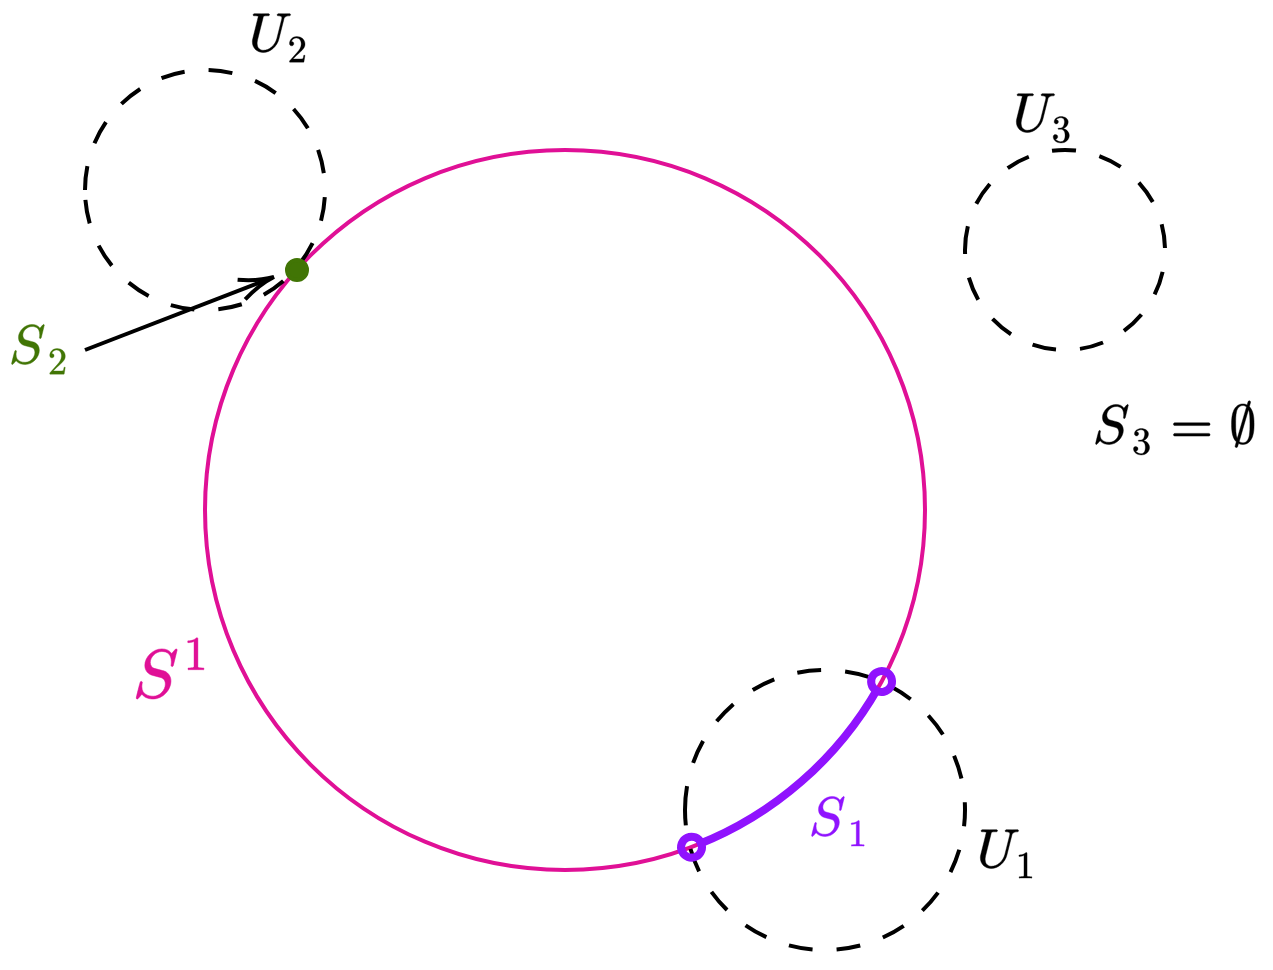
\includegraphics[width=0.35\textwidth]{lec04-1_sphere.png}
			      \caption{1-sphere induced topology}
			      \label{fig:1-sphere_induced_topology}
		      \end{figure} \noindent
		      From \cref{fig:1-sphere_induced_topology}, we can see that \(U_i\)'s are open in \(\R^2\) and \(U_i \cap S^1\) are open in \(S^1\). See, \(U_3 \in \Ostd \implies \0 \in \O\) and \(U_1 \in \Ostd \implies S_1 \in \O\). Also, the set \(S_2\) is not open in \(S^1\) as \(\forall U \in \powerset(\R): U \cap S^1 \neq S_2\). Hence, \(S_2 \notin \O\).

		\item \uline{Quotient Topology:} Let $\sim$ be the equivalence relation on $\R$ defined by:
		      \begin{equation*}
			      x \sim y :\iff \exists n \in \Z : x = y + 2 \pi n.
		      \end{equation*}
		      Then the circle can be defined as the set $S^1 := \faktor{\R}{\sim}$ equipped with the quotient topology.
	\end{enumerate}
\end{example}

\subsection{Product Topology}

\begin{definition}[Product Topology]
	Let \((A, \O_A)\) and \((B, \O_B)\) be two topological spaces. Then the set \(\O_{A \times B}\) defined implicitly as
	\begin{equation}
		U \in \O_{A \times B} :\iff \forall (a, b) \in U: \exists U_A \in \O_A, U_B \in \O_B: a \in U_A \land b \in U_B \land U_A \times U_B \subseteq U \label{eq:product_topology}
	\end{equation}
	is a topology on \(A \times B\), called the \emph{product topology} on \(A \times B\).
\end{definition}
Here we used the existence of \(U_A\) and \(U_B\) such that it contains \(a\) and \(b\) respectively. And we will use this kind of argument throughout our discussion.

\noindent Let \((M, \O)\) be a topological space. Let \(a \in M\) be a point. Then we say that a set \(U \in \O\) is an \emph{open neighbourhood} of \(a\) if \(a \in U\).

Intuitively, the definition can be understood with the help of following diagram:
\begin{figure}[H]
	\centering
	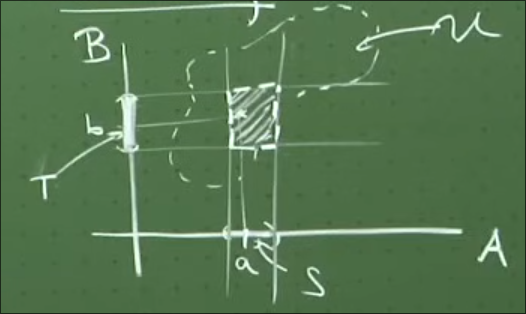
\includegraphics[width=0.375\textwidth]{lec04-prod_topology_intuition.png}
	% \caption{Product Topology Intuition}
	\label{fig:prod_topology_intuition}
\end{figure}

\begin{remark}[Extending product topology to finite cartesian product]
	Let \(A_1, A_2, \ldots, A_N\) be topological spaces. Then in same spirit, we can define the product topology
	\begin{equation*}
		\O_{A_1 \times A_2 \times \cdots \times A_N}
	\end{equation*}
\end{remark}
With this, we can check that the standard topology on \(\R^d\) is a product topology with open ball defined using \(\norm{\cdot}_{\infty}\)
\begin{equation*}
	\Ostd {\;}_{\R^d} = \O_{\underbrace{\R \times \R \times \cdots \times \R}_{d\ \text{times}}}
\end{equation*}

Till this point, we have seen topology and topological spaces from geometric view-point. But one can use these things beyond the geometric (or manifold) applications. For example, a guy named Furstenberg introduced a simple topology on the set of integers to prove the infinitude of primes.

\section{Convergence}

\begin{definition}[Sequence]
	A \emph{sequence} (of points) in a set \(M\) is a map from \(\N\) onto \(M\), \ie\ \(q: \N \to M\).
\end{definition}

\begin{definition}[Convergence and Limit Point]
	Let \((M, \O)\) be a topological space. A sequence \(q\) in \(M\) is said to \emph{converge} against a \emph{limit point} \(a \in M\) if
	\begin{equation}
		\forall U \in \O: a \in U \implies \exists N \in \N: \forall n > N: q(n) \in U \label{eq:convergence}
	\end{equation}
\end{definition}

\begin{example}[Justifying different topologies]
	With the notion of convergence, we can justify the different topologies on a set.
	\begin{enumerate}[(a)]
		\item \uline{Chaotic Topology:} Consider the chaotic topology \(\O = \qty{\0, M}\) on \(M\). Then any sequence in \(M\) converges against any point in \(M\). Let \(a \in M\) and \(q\) be a sequence in \(M\), then we have only two choice for \(U \in \O\), \ie\ \(U = \0\) or \(U = M\). In case \(U = \0\), the definition of convergence is vacuously true. In case \(U = M\), the definition of convergence is true as \(q(n) \in M\) for all \(n \in \N\). Hence, (arbitrary) sequence \(q\) converges against (arbitrary) point \(a\) in \((M, \O)\).

		      This weird behavior is the reason for the name ``chaotic topology''.

		\item \uline{Discrete Topology:} Consider the discrete topology \(\O = \powerset(M)\) on \(M\). Then only almost constant sequences converge against a (unique) point in \(M\). Let \(a \in M\) and \(q\) be a sequence in \(M\), then we have \(U = \qty{a} \in \O\). Then the definition of convergence is true if and only if \(q(n) = a\) for all \(n > N\). Hence, only almost constant sequences converge against a point in \((M, \O)\).
	\end{enumerate}
\end{example}

Here we can see that every sequence is convergent in chaotic topology (the coarsest topology) and only a specific kind of sequence is convergent in discrete topology (the finest topology). So we deduce the following remark.

\begin{remark}\label{rem:convergence_in_comparison_topologies}
	Let \(M\) be a set and \(\O_1, \O_2\) be two topologies on \(M\) such that \(\O_1 \subseteq \O_2\) and let \(q\) be a sequence in \(M\). Then if \(q\) converges in \((M, \O_2)\), then \(q\) converges in \((M, \O_1)\) but not necessarily vice-versa.
\end{remark}

\begin{theorem}[Convergence in standard topology on \(\R^d\)]
	Let \(q\) be a sequence in \(\R^d\) and \(a \in \R^d\). Then \(q\) converges against \(a\) in \((\R^d, \Ostd)\) if and only if
	\begin{equation}
		\forall \eps > 0: \exists N \in \N: \forall n > N: \norm{q(n) - a} < \eps \label{eq:convergence_Rd}
	\end{equation}
\end{theorem}

\begin{proof}
	Let \(q\) be a sequence in \(\R^d\) and \(a \in \R^d\). Then \(q\) converges against \(a\) in \((\R^d, \Ostd)\) if and only if
	\begin{equation}
		\forall U \in \Ostd: a \in U \implies \exists N \in \N: \forall n > N: q(n) \in U \label{eq:convergence_Rd_1}
	\end{equation}
	From the definition of standard topology on \(\R^d\), we have \(U \in \Ostd \implies \exists r \in \R^+: B_r(a) \subseteq U\). Hence, \eqref{eq:convergence_Rd_1} is equivalent to
	\begin{equation}
		\forall r > 0: \exists N \in \N: \forall n > N: q(n) \in B_r(a) \label{eq:convergence_Rd_2}
	\end{equation}
	which is equivalent to \eqref{eq:convergence_Rd}.
\end{proof}

\begin{example}[Convergence in \(\R\)]
	Let \(q(n) = 1 - \frac{1}{n + 1}\) be a sequence in \(\R\). Then \(q\) converges against \(1\) in \((\R, \Ostd)\) as
	\begin{equation*}
		\forall \eps \in \R^+: \exists N \in \N: \forall n > N: \abs{q(n) - 1} = \abs{1 - \frac{1}{n + 1} - 1} = \frac{1}{n + 1} < \eps
	\end{equation*}
	But observe \(q\) is not almost constant sequence and hence does not converge in \((\R, \powerset(\R))\).
\end{example}

\section{Continuity}

\begin{definition}[Continuity]
	Let \((M, \O_M)\) and \((N, \O_N)\) be two topological spaces and \(\phi: M \to N\) be a map. Then \(\phi\) is said to be \emph{continuous} if
	\begin{equation}
		\forall V \in \O_N: \preimg_{\phi}(V) \in \O_M \label{eq:continuity}
	\end{equation}
	In other words, \(\phi\) is continuous iff the pre-image of every open set in \(N\) is open in \(M\).
\end{definition}

\begin{example}[`Trivial' Continuity]
	Let \((M, \O_M)\) and \((N, \O_N)\) be two topological spaces and \(\phi: M \to N\) be a map. Then
	\begin{enumerate}[(a)]
		\item Let \(\O_M = \powerset(M)\) and \(\O_N\) be any topology on \(N\). Then every map is continuous.

		      Let \(V \in \O_N\) be any open set in \(N\). Then \(\preimg_{\phi}(V) \subseteq M\) and hence \(\preimg_{\phi}(V) \in \O_M\). Hence, \(\phi\) is continuous.

		\item Let \(\O_M\) be any topology on \(M\) and \(\O_N = \qty{\0, N}\). Then every map is continuous.

		      Here, either \(V = \0\) or \(V = N\). In case \(V = \0\), we have \(\preimg_{\phi}(\0) = \0 \in \O_M\). In case \(V = N\), we have \(\preimg_{\phi}(N) = M \in \O_M\). Hence, \(\phi\) is continuous.
	\end{enumerate}
\end{example}

Recovering the definition of \(\eps-\delta\) definition of continuity on `Euclidean' spaces from the definition of continuity in topological spaces.
\begin{theorem}[Continuity in Euclidean spaces]
	Let \(f: \R^m \to \R^n\) be a map. Then \(f\) is continuous if and only if
	\begin{equation}
		\forall a \in \R^m: \forall \eps > 0: \exists \delta > 0: \norm{x - a} < \delta \implies \norm{f(x) - f(a)} < \eps \label{eq:continuity_Rm_Rn}
	\end{equation}
\end{theorem}

\begin{proof}
	Let \(f: \R^m \to \R^n\) be a map. Then \(f\) is continuous if and only if
	\begin{equation}
		\forall U \in \O_{\R^n}: \preimg_{f}(U) \in \O_{\R^m} \label{eq:continuity_Rm_Rn_1}
	\end{equation}
	From the definition of standard topology on \(\R^n\), we have \(U \in \O_{\R^n} \implies \exists \eps > 0: B_{\eps}(f(a)) \subseteq U\). Hence, \eqref{eq:continuity_Rm_Rn_1} is equivalent to
	\begin{equation}
		\forall \eps > 0: \exists \delta > 0: \preimg_{f}(B_{\eps}(f(a))) \in \O_{\R^m} \label{eq:continuity_Rm_Rn_2}
	\end{equation}
	which is equivalent to \eqref{eq:continuity_Rm_Rn}.
\end{proof}

\subsection{Homeomorphism}

\begin{definition}[Homeomorphism]
	Let \((M, \O_M)\) and \((N, \O_N)\) be two topological spaces. Let \(\phi: M \to N\) be a bijection. Then \(\phi\) is said to be a \emph{homeomorphism} if
	\begin{enumerate}[(a)]
		\item \(\phi\) is continuous, and
		\item \(\phi^{-1}\) is continuous.
	\end{enumerate}
\end{definition}

\begin{remark}[Structure preserving maps]
	Homeomorphisms are structure preserving maps in topology.
\end{remark}

\begin{remark}[One-to-one pairing of open sets]
	Let \((M, \O_M)\) and \((N, \O_N)\) be two topological spaces and let \(\phi: M \to N\) be a homeomorphism.
	\begin{figure}[H]
		\centering
		\begin{tikzcd}
			M \arrow[r, bend left, "\phi"] & N \arrow[l, bend left, "\phi^{-1}"]
		\end{tikzcd}
	\end{figure}
	Then \(\phi\) provides a \emph{one-to-one} pairing of the open sets of \(M\) with those of \(N\).
\end{remark}

\begin{definition}[Homeomorphic]
	Let \((M, \O_M)\) and \((N, \O_N)\) be two topological spaces. Then \(M\) and \(N\) are said to be \emph{homeomorphic} if there exists a homeomorphism between them. And we write
	\begin{equation}
		M \topIso N \label{eq:homeomorphic}
	\end{equation}
\end{definition}

\begin{remark}[Homeomorphic \& Isomorphic]
	Let \((M, \O_M)\) and \((N, \O_N)\) be two homeomorphic topological spaces. Then they are isomorphic as sets. But the converse is not true.
	\begin{equation}
		M \topIso N \implies M \setIso N \label{eq:homeomorphic_isomorphic}
	\end{equation}
\end{remark}

\lecture{5}

In case of set theory, we had a notion of `cardinality' of a set. With the help of this notion, we can say that if two sets are isomorphic (set theoretically) then they have the same cardinality. But in case of topological spaces, we don't have any such quantity \ie\ we don't have any property which can tell us that two topological spaces are `homeomorphic' or not.

Building on this idea, we had classified sets into different types based on their cardinality like finite, countable, uncountable, etc. But in case of topology, classification of topological spaces is an open problem.

\section{Topological Properties I: Separation Axioms}

\begin{definition}[T1 Space]\label{def:t1_space}
	A topological space \((M, \O)\) is called \emph{T1} if for any two distinct points \(p, q \in M\) (\ie\ \(p \neq q\)), then
	\begin{equation}
		\exists U_p \in \O: q \notin U_p \label{eq:separation_axiom_t1}
	\end{equation}
	here \(U_p\) is an open neighbourhood of \(p\).
\end{definition}

\begin{definition}[T2 Space]\label{def:t2_space}
	A topological space \((M, \O)\) is called \emph{T2} or \emph{Hausdorff} if for any two distinct points \(p, q \in M\) (\ie\ \(p \neq q\)), then
	\begin{equation}
		\exists U_p, V_q \in \O: U_p \cap V_q = \0 \label{eq:separation_axiom_t2}
	\end{equation}
	here \(U_p\) and \(V_q\) are open neighbourhoods of \(p\) and \(q\) respectively.
\end{definition}
Intuitively, we can see why \cref{def:t1_space} and \cref{def:t2_space} are called `separation axioms'. Consider standard topology on \(\R^2\), see \cref{fig:separation_axioms}.
\begin{figure}[H]
	\centering
	\begin{subfigure}{0.45\textwidth}
		\centering
		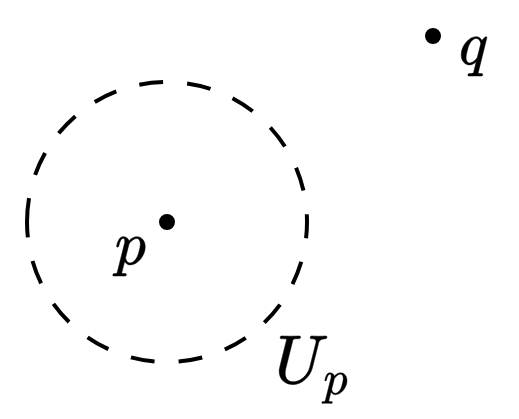
\includegraphics[width=0.5\linewidth]{lec05-t1_intuition.png}
		\caption{T1 Space}
		\label{fig:t1_space}
	\end{subfigure}
	\begin{subfigure}{0.45\textwidth}
		\centering
		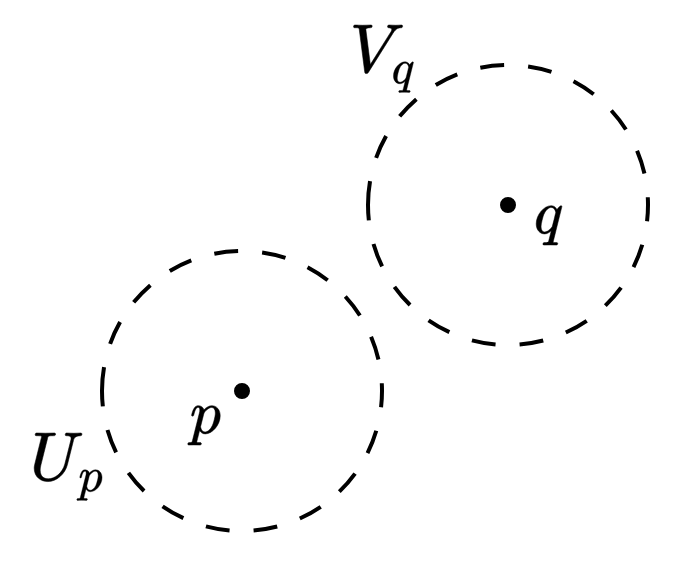
\includegraphics[width=0.6\linewidth]{lec05-t2_intuition.png}
		\caption{T2 Space}
		\label{fig:t2_space}
	\end{subfigure}
	\caption{Separation Axioms}
	\label{fig:separation_axioms}
\end{figure}

\begin{remark}[T1 vs T2]
	Every T2 space is a T1 space, but the converse is not true.
\end{remark}

\begin{example}
	Some examples of topological spaces based on separation axioms are:
	\begin{enumerate}[(a)]
		\item \(\R^d\) with standard topology is a T2 space.
		\item Zariski topology (algebraic geometry) is T1 but not T2.
		\item Chaotic topology is neither T1 nor T2.
		\item Discrete topology is always T1 and T2.
	\end{enumerate}
\end{example}


There are many other ``T'' properties, like T3, T4, etc. All of them have use cases in some area of mathematics or physics.
\begin{remark}[T$2\frac{1}{2}$ Space]
	A topological space \((M, \O)\) is called \emph{T$2\frac{1}{2}$} if for any two distinct points \(p, q \in M\) (\ie\ \(p \neq q\)), then there exists a closed neighbourhood \(U_p\) of \(p\) such that \(q \notin U_p\).
\end{remark}

\begin{theorem}[Uniqueness of Limit Point]\label{thm:uniqueness_limit_point}
	Let \((M, \O)\) be a Hausdorff space. Then every convergent sequence in \(M\) has a unique limit point.
\end{theorem}

\section{Compactness and Paracompactness}

Before we define compactness, we need to understand the concept of `open cover'.

\begin{definition}[Cover and Open Cover]\label{def:cover}
	Let \((M, \O)\) be a topological space. A set \(C \subseteq \powerset(M)\) is called a \emph{cover} of \(M\) if
	\begin{equation}
		\bigcup C = M. \label{eq:cover}
	\end{equation}
	If \(C \subseteq \O\) then it is called an \emph{open cover}.
\end{definition}

\begin{definition}[Subcover and Finite Subcover]\label{def:subcover}
	Let \(C\) be a cover of \(M\). A subset \(\tilde{C} \subseteq C\) is called a \emph{subcover} of \(C\) if
	\begin{equation}
		\bigcup \tilde{C} = M. \label{eq:subcover}
	\end{equation}
	If \(\tilde{C}\) is finite then it is called a \emph{finite subcover}.
\end{definition}

\subsection{Compactness}
\begin{definition}[Compact Space]\label{def:compact_space}
	A topological space \((M, \O)\) is called \emph{compact} if every open cover of \(M\) has a finite subcover.
\end{definition}

It is clear from the definition that compactness is a topological property. So we have,
\begin{remark}
	Let \((M, \O_M)\) and \((N, \O_N)\) be two homeomorphic topological spaces. Then \(M\) is compact if and only if \(N\) is compact.
\end{remark}

\begin{definition}[Compact Subset]\label{def:compact_subset}
	Let \((M, \O)\) be a topological space. A subset \(N \subseteq M\) is called \emph{compact} if the induced topology \((N, \eval{\O}_N)\) is compact.
\end{definition}

Determining whether a topological space is compact or not, is not an easy task. With the help of a suitable homeomorphism we can simplify this task.

\begin{theorem}[Heine-Borel Theorem]\label{thm:heine_borel}
	Let \((\R^d, \Ostd)\) be a topological space. Then a subset \(K \subseteq \R^d\) is compact if and only if it is closed and bounded.
\end{theorem}

\begin{remark}[Bounded Set in \(\R^d\)]
	A set \(K \subseteq \R^d\) is called \emph{bounded} if
	\begin{equation}
		\exists r > 0: K \subseteq B_r(0) \label{eq:bounded_set}
	\end{equation}
\end{remark}

We can extend \nameref{thm:heine_borel} to any metric space. But first we need to define the concept of `metric space'.

\begin{definition}[Metric Space]
	Let \(M\) be a set. A function \(d: M \times M \to \R\) is called a \emph{metric} on \(M\) if it satisfies the following properties for all \(p, q, r \in M\):
	\begin{itemize}
		\item \uline{\emph{Symmetry}:} \(d(p, q) = d(q, p)\).
		\item \uline{\emph{Positivity}:} \(d(p, q) \geq 0\) and \(d(p, q) = 0 \iff p = q\).
		\item \uline{\emph{Triangle Inequality}:} \(d(p, q) + d(q, r) \geq d(p, r)\).
	\end{itemize}
	A set \(M\) equipped with a metric \(d\) is called a \emph{metric space}.
\end{definition}

We can define `metric-induced topology' on a metric space as we did for \(\R^d\).

\begin{remark}[Metric-Induced Topology]
	Let \((M, d)\) be a metric space. Then the set \(B_r(p)\) is an open ball of radius \(r \in \R^+\) centered at \(p \in M\) defined as
	\begin{equation}
		B_r(p) = \{q \in M: d(p, q) < r\}. \label{eq:open_ball}
	\end{equation}
	With this, we can define the metric-induced topology \(\O_d\) on \(M\) as
	\begin{equation}
		U \in \O_d :\iff \forall p \in U, \exists r \in \R^+: B_r(p) \subseteq U. \label{eq:metric_induced_topology}
	\end{equation}
\end{remark}

\begin{theorem}[Generalized Heine-Borel Theorem]\label{thm:generalized_heine_borel}
	Let \((M, d)\) be a metric space with metric-induced topology \(\O_d\). Then a subset \(K \subseteq M\) is compact if and only if it is \emph{complete} and \emph{totally bounded}.
\end{theorem}

\begin{example}
	Example of compact subsets in \(\R\) are:
	\begin{enumerate}[(a)]
		\item \([0, 1]\) is compact in \((\R, \Ostd)\).

		\item \(\R\) is not compact in \((\R, \Ostd)\). It suffices to show that there exists an open cover of \(\R\) which does not have a finite subcover. Consider the open cover
		      \begin{equation}
			      C := \qty{(n, n + 1) \mid n \in \Z} \cup \qty{(n + \fhalf, n + \flatfrac{3}{2}) \mid n \in \Z}.
		      \end{equation}
	\end{enumerate}
\end{example}

\noindent We can prove that the product of two compact spaces is compact for product topology.
\begin{theorem}
	Let \((M, \O_M)\) and \((N, \O_N)\) be two compact topological spaces. Then the product space \((M \times N, \O_{M \times N})\) is compact.
\end{theorem}
Now extending this to finite product spaces is easy.

Compactness is a very strong property, and sometimes it doesn't hold. So we need a weaker property which can be used in such cases. This is where the concept of `paracompactness' comes in.

\subsection{Paracompactness}

\begin{definition}[Refinement of a Cover]\label{def:refinement_cover}
	Let \(C\) be a cover of \(M\). A cover \(R\) of \(M\) is called a \emph{refinement} of \(C\) if
	\begin{equation}
		\forall \tilde{U} \in R: \exists U \in C: \tilde{U} \subseteq U. \label{eq:refinement_cover}
	\end{equation}
	A refinement \(R\) is said to be:
	\begin{itemize}
		\item \emph{open} if \(R \subseteq \O\).
		\item \emph{Locally finite} if for every \(p \in M\), there exists an open neighbourhood \(U_p\) of \(p\) such that
		      \begin{equation}
			      \abs{\qty{\tilde{U} \in R \mid \tilde{U} \cap U_p \neq \0}} < \infty. \label{eq:locally_finite_cover}
		      \end{equation}
	\end{itemize}
\end{definition}

\begin{remark}
	Let \(C\) be a cover of \(M\) and let \(\tilde{C}\) be a subcover of \(C\). Then \(\tilde{C}\) is a refinement of \(C\). But the converse is not true.
\end{remark}

\begin{definition}[Paracompact Space]\label{def:paracompact_space}
	A topological space \((M, \O)\) is called \emph{paracompact} if every open cover of \(M\) has a locally finite open refinement.
\end{definition}

\begin{corollary}
	Every compact space is paracompact.
\end{corollary}

\begin{definition}[Metrisable Space]
	A topological space \((M, \O)\) is called \emph{metrizable} if there exists a metric \(d\) on \(M\) such that the metric-induced topology \(\O_d\) is same as \(\O\).
\end{definition}

\begin{theorem}[Stone's Theorem]\label{thm:stone}
	Every metrizable space is paracompact.
\end{theorem}

\begin{example}
	Let's see some topological spaces which are paracompact or not:
	\begin{enumerate}[(a)]
		\item The topological space \((\R^d, \Ostd)\) is metrizable since \(\Ostd = \O_d\) where \(d = \norm{\cdot}_2\). Hence, \((\R^d, \Ostd)\) is paracompact.
		\item Alexandroff Long Line is not paracompact. To construct it, we first observe that we could ``build'' \(\R\) by taking the interval \([0,1)\) and stacking countably many copies of it one after the other. Hence, in a sense, \(\R\) is equivalent to \(\Z \times [0,1)\). The long line \(L\) is defined analogously as \(L: \omega_1 \times [0,1)\), where \(\omega_1\) is an uncountable infinite set. The resulting space \(L\) is not paracompact.
	\end{enumerate}
\end{example}

\begin{theorem}
	Let \((M, \O)\) be a paracompact space and \((N, \O_N)\) be a compact space. Then the product space \((M \times N, \O_{M \times N})\) is paracompact.
\end{theorem}

\begin{corollary}
	Let \((M, \O)\) be a paracompact space and \((N_i, \O_{N_i})\) be compact spaces for all \(i \in \qty{1, 2, \ldots, n}\). Then the product space \(M \times N_1 \times N_2 \times \ldots \times N_n\) is paracompact.
\end{corollary}

At this point, we can discuss the sufficient and necessary criteria for paracompactness which are used as definitions in some books. For that we need to define the concept of `\emph{partition of unity}.'

\begin{definition}[Partition of Unity]\label{def:partition_of_unity}
	Let \((M, \O)\) be a topological space. A set \(\mathcal{F}\) of continuous functions \(\phi: M \to [0, 1]\) is called a \emph{partition of unity} if for each \(p \in M\),
	\begin{enumerate}[(a)]
		\item There exists an open neighbourhood \(U_p\) such that \(\phi(p) \ne 0\) for finitely many \(\phi \in \mathcal{F}\).
		\item \(\sum\limits_{\phi \in \mathcal{F}} \phi(p) = 1\).
	\end{enumerate}
\end{definition}

\begin{definition}[Partition of Unity Subordinate to a Cover]\label{def:partition_of_unity_subordinate}
	Let \((M, \O)\) be a topological space and let \(C\) be a cover of \(M\). A partition of unity \(\mathcal{F}\) is said to be \emph{subordinate} to \(C\) if:
	\begin{equation}
		\forall \phi \in \mathcal{F}: \exists U \in C: f(p) \ne 0 \implies p \in U. \label{eq:partition_of_unity_subordinate}
	\end{equation}
\end{definition}

\begin{theorem}
	Let \((M, \O)\) be a Hausdorff space. Then \(M\) is paracompact if and only if every open cover \(C\) admits a partition of unity subordinate to \(C\).
\end{theorem}

\begin{example}
	Let \((\R, \Ostd)\) be a topological space. By \cref{thm:stone}, \((\R, \Ostd)\) is paracompact. Consider the open cover \(C := \qty{U_1 = (-\infty, 1), U_2 = (0, \infty)}\). We can construct a partition of unity \(\mathcal{F} = \qty{\phi_1, \phi_2}\) subordinate to \(C\) as follows:
	\begin{align*}
		\phi_1(x) = \begin{cases}
			            1       & \text{if}\ x \le 0       \\
			            1 - x^2 & \text{if}\ 0 \le x \le 1 \\
			            0       & \text{if}\ x \ge 1
		            \end{cases} \qquad \text{and} \qquad
		\phi_2(x) = \begin{cases}
			            0   & \text{if}\ x \le 0       \\
			            x^2 & \text{if}\ 0 \le x \le 1 \\
			            1   & \text{if}\ x \ge 1
		            \end{cases}
	\end{align*}
	For \(\phi_1\), we have \(U_1 = (-\infty, 1)\) for which \(\phi_1(x) \ne 0\) and for \(\phi_2\), we have \(U_2 = (0, \infty)\) for which \(\phi_2(x) \ne 0\). Also, \(\phi_1(x) + \phi_2(x) = 1\) for all \(x \in \R\).
\end{example}

\section{Connectedness and Path-Connectedness}

\subsection{Connectedness}
\begin{definition}[Connected Space]\label{def:connected_space}
	A topological space \((M, \O)\) is called \emph{connected} unless there exists two non-empty open sets \(A, B\) such that
	\begin{equation}
		A \cup B = M \quad \text{and} \quad A \cap B = \0. \label{eq:connected_space}
	\end{equation}
\end{definition}

\begin{example}
	Let \(\qty(M := \R \setminus \qty{0}, \O := \eval{\Ostd}_{\R \setminus \qty{0}})\) be a topological space. Then \(M\) is not connected since we can write \(M = A \cup B\) where \(A = (-\infty, 0)\) and \(B = (0, \infty)\) with \(A \cap B = \0\).
\end{example}

\begin{theorem}
	The closed interval \([0, 1]\) with induced topology from \((\R, \Ostd)\) is connected.
\end{theorem}

\begin{theorem}
	Let \((M, \O)\) be a topological space. Then \(M\) is connected if and only if \(\0\) and \(M\) are the only subsets of \(M\) that are both open and closed.
\end{theorem}

\begin{proof}

	[\(\implies\)]:\\
	Suppose not there exists a set \(U \subseteq M\) that is both open and closed and \(U \neq \0, M\). Then \(M = U \dcup (M \setminus U)\). Since \(U\) is open and \(M \setminus U\) is open (as \(U\) is closed). Hence, \(M\) is not connected. \(\contra\)

	\noindent [\(\impliedby\)]:\\
	Suppose not \(M\) is not connected. Then there exists two non-empty open sets \(A, B\) such that \(A \cup B = M\) and \(A \cap B = \0\). Clearly, \(A \ne M\), if not then \(B = \0\). Since \(A\) is open, \(M \setminus A\) is closed. But \(M \setminus A = B\) is also open. Hence, \(B \ne \0, M\) is open and closed. \(\contra\)
\end{proof}

\subsection{Path-Connectedness}
\begin{definition}[Path-Connected Space]\label{def:path_connected_space}
	A topological space \((M, \O)\) is called \emph{path-connected} if for every pair of points \(p, q \in M\), there exists a continuous curve \(\gamma: [0, 1] \to M\) such that \(\gamma(0) = p\) and \(\gamma(1) = q\).
\end{definition}

\begin{example}
	Let \((\R^d, \Ostd)\) be a topological space. Then \((\R^d, \Ostd)\) is path-connected.
\end{example}
\begin{proof}
	Let \(p, q \in \R^d\). Then the curve \(\gamma(\lambda) := (1 - \lambda)p + \lambda q\) is continuous and \(\gamma(0) = p\) and \(\gamma(1) = q\).
\end{proof}

\begin{example}
	Let \(S := \qty{\qty(x, \sin(\frac{1}{x})) \mid x \in (0, 1]} \cup \qty{(0, 0)} \subseteq \R^2\). Then \((S, \eval{\Ostd}_{S})\) is not path-connected but connected.
	\begin{figure}[H]
		\centering
		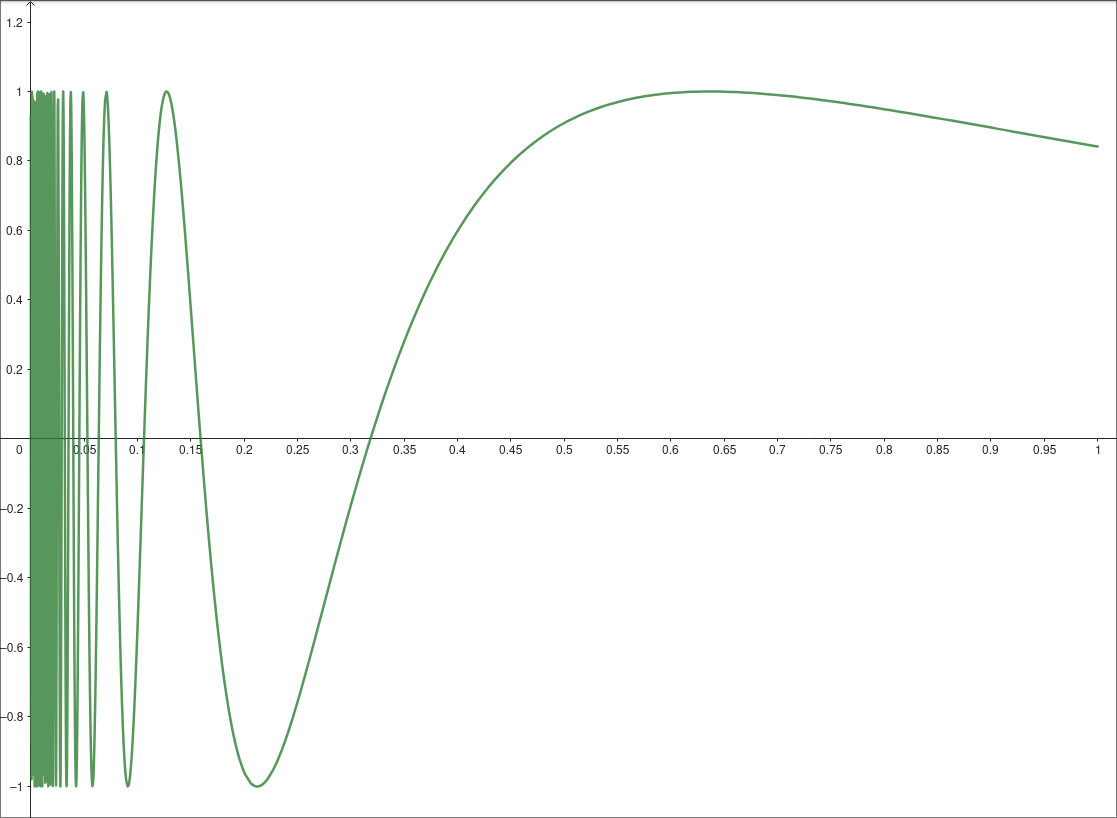
\includegraphics[width = 0.7\textwidth]{lec05-eg_path_connected.png}
		% \caption{}
		% \label{fig:}
	\end{figure}
\end{example}

\begin{theorem}
	Every path-connected space is connected.
\end{theorem}
\begin{proof}
	Let \((M, \O)\) be a path-connected space. Suppose not \(M\) is not connected. Then there exists two non-empty open sets \(A, B\) such that \(A \dcup B = M\). Since, \(A\) and \(B\) are non-empty, we can choose \(a \in A\) and \(b \in B\). Since \(M\) is path-connected, there exists a continuous curve \(\gamma: [0, 1] \to M\) such that \(\gamma(0) = a\) and \(\gamma(1) = b\). Moreover, \(\gamma\) is continuous and \(A, B\) are open, disjoint sets, \(\preimg_{\gamma}(A)\) and \(\preimg_{\gamma}(B)\) are open, disjoint sets. We know
	\begin{equation*}
		\qty[0, 1] = \preimg_{\gamma}(M) = \preimg_{\gamma}(A \dcup B) = \preimg_{\gamma}(A) \dcup \preimg_{\gamma}(B).
	\end{equation*}
	Thus, existence of \(\preimg_{\gamma}(A)\) and \(\preimg_{\gamma}(B)\) implies that \([0, 1]\) is not connected. \(\contra\)
\end{proof}

\section{Homotopic Curves and Fundamental Group}

\begin{definition}[Homotopic Curves]\label{def:homotopic_curves}
	Let \((M, \O)\) be a topological space. Two continuous curves \(\gamma_1, \gamma_2: [0, 1] \to M\) such that
	\begin{equation*}
		\gamma_1(0) = \gamma_2(0) \quad \text{and} \quad \gamma_1(1) = \gamma_2(1)
	\end{equation*}
	are called \emph{homotopic} if there exists a continuous function \(h: [0, 1] \times [0, 1] \to M\) such that for all \(\lambda \in [0, 1]\),
	\begin{equation}
		h(0, \lambda) = \gamma_1(\lambda) \quad \text{and} \quad h(1, \lambda) = \gamma_2(\lambda). \label{eq:homotopic_curves}
	\end{equation}
\end{definition}
\uline{Intuitively}, two curves are homotopic if one can be continuously deformed into the other.\\
Pictorially, see \cref{fig:homotopic_curves}.
\begin{figure}[H]
	\centering
	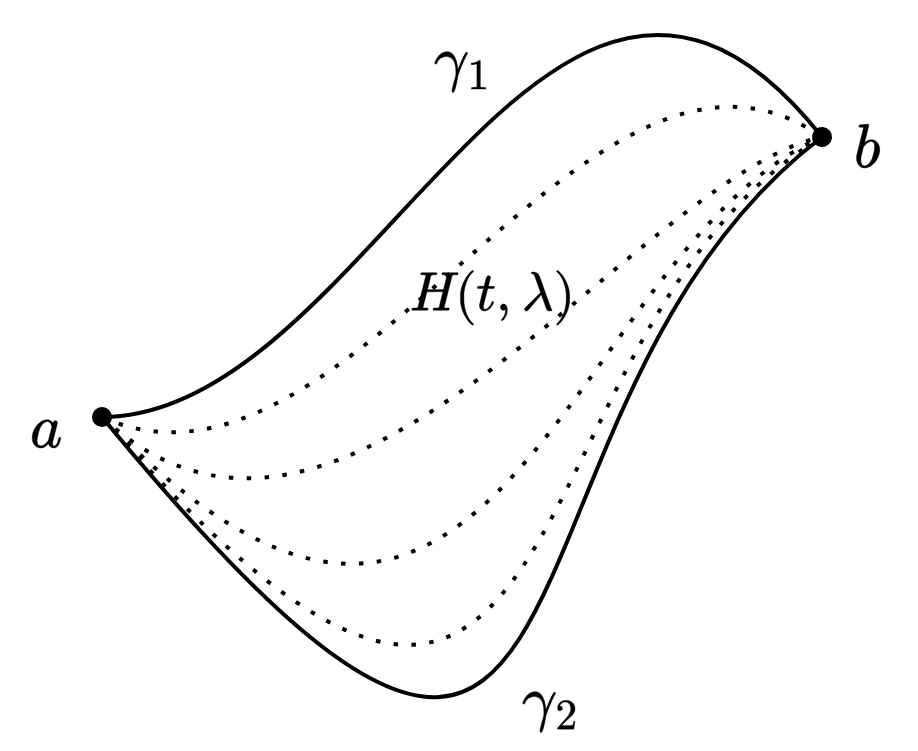
\includegraphics[width=0.4\textwidth]{lec05-homotopic_curves.png}
	\caption{Homotopic Curves}
	\label{fig:homotopic_curves}
\end{figure}

\begin{proposition}[Homotopy is an Equivalence Relation]\label{prop:homotopy_equivalence_relation}
	Let \((M, \O)\) be a topological space. Define a relation \(\sim\) on the set of continuous curves \(\qty{\gamma: [0, 1] \to M}\) by
	\begin{equation}
		\gamma_1 \sim \gamma_2 :\iff \gamma_1 \text{ and } \gamma_2 \text{ are homotopic}. \label{eq:homotopy_equivalence_relation}
	\end{equation}
	Then \(\sim\) is an equivalence relation.
\end{proposition}
\begin{proof}
	Let \(\gamma_1, \gamma_2, \gamma_3: [0, 1] \to M\) be continuous curves.
	\begin{enumerate}[(a)]
		\item \uline{Reflexivity:} Define a continuous function \(h: [0, 1] \times [0, 1] \to M\) as \(h(t, \lambda) := \gamma_1(\lambda)\). Then \(h(0, \lambda) = \gamma_1(\lambda)\) and \(h(1, \lambda) = \gamma_1(\lambda)\) for all \(\lambda \in [0, 1]\). Hence, \(\gamma_1 \sim \gamma_1\).
		\item \uline{Symmetry:} Let \(\gamma_1 \sim \gamma_2\). Then there exists a continuous function \(h: [0, 1] \times [0, 1] \to M\) such that \(h(0, \lambda) = \gamma_1(\lambda)\) and \(h(1, \lambda) = \gamma_2(\lambda)\) for all \(\lambda \in [0, 1]\). Define a continuous function \(h': [0, 1] \times [0, 1] \to M\) as \(h'(t, \lambda) := h(1 - t, \lambda)\). Then \(h'(0, \lambda) = \gamma_2(\lambda)\) and \(h'(1, \lambda) = \gamma_1(\lambda)\) for all \(\lambda \in [0, 1]\). Hence, \(\gamma_2 \sim \gamma_1\).
		\item \uline{Transitivity:} Let \(\gamma_1 \sim \gamma_2\) and \(\gamma_2 \sim \gamma_3\). Then there exists continuous functions \(h_1, h_2: [0, 1] \times [0, 1] \to M\) such that \(h_1(0, \lambda) = \gamma_1(\lambda)\), \(h_1(1, \lambda) = \gamma_2(\lambda)\) and \(h_2(0, \lambda) = \gamma_2(\lambda)\), \(h_2(1, \lambda) = \gamma_3(\lambda)\) for all \(\lambda \in [0, 1]\). Define a continuous function \(h: [0, 1] \times [0, 1] \to M\) as
		      \begin{equation}
			      h(t, \lambda) := \begin{cases}
				      h_1(2t, \lambda)     & \text{if}\ 0 \le t \le \frac{1}{2} \\
				      h_2(2t - 1, \lambda) & \text{if}\ \frac{1}{2} \le t \le 1
			      \end{cases}
		      \end{equation}
		      Then \(h(0, \lambda) = \gamma_1(\lambda)\) and \(h(1, \lambda) = \gamma_3(\lambda)\) for all \(\lambda \in [0, 1]\). Hence, \(\gamma_1 \sim \gamma_3\).
	\end{enumerate}
\end{proof}

\begin{definition}[Space of Loops]\label{def:space_of_loops}
	Let \((M, \O)\) be a topological space. Then, for every point \(p \in M\), the set \(\mathscr{L}_p\) defined as
	\begin{equation}
		\mathscr{L}_p := \qty{\gamma: [0, 1] \to M \mid \gamma \ \text{is continuous and}\ \gamma(0) = \gamma(1) = p} \label{eq:space_of_loops}
	\end{equation}
	is called the \emph{space of loops} at \(p\).
\end{definition}

\begin{definition}[Concatenation of Loops]\label{def:concatenation_of_loops}
	Let \((M, \O)\) be a topological space. Fix a point \(p \in M\). We define the \emph{concatenation} operation \(\ast_p: \mathscr{L}_p \times \mathscr{L}_p \to \mathscr{L}_p\) as
	\begin{equation}
		(\gamma_1 \ast_p \gamma_2)(\lambda) := \begin{cases}
			\gamma_1(2\lambda)     & \text{if}\ 0 \le \lambda < \frac{1}{2}   \\
			\gamma_2(2\lambda - 1) & \text{if}\ \frac{1}{2} \le \lambda \le 1
		\end{cases} \label{eq:concatenation_of_loops}
	\end{equation}
\end{definition}

\subsection{Fundamental Group}

We will first recall the definition of a group.
\begin{definition}[Group]\label{def:group}
	A set \(G\) equipped with a binary operation \(\ast: G \times G \to G\) is called a \emph{group} if it satisfies the following properties:
	\begin{enumerate}[(a)]
		\item \uline{\emph{Associativity}:} \(\forall a, b, c \in G: (a \ast b) \ast c = a \ast (b \ast c)\).
		\item \uline{\emph{Identity Element}:} \(\exists e \in G: \forall a \in G: a \ast e = e \ast a = a\).
		\item \uline{\emph{Inverse Element}:} \(\forall a \in G: \exists a^{-1} \in G: a \ast a^{-1} = a^{-1} \ast a = e\).
	\end{enumerate}
	A group is called \emph{abelian} (or \emph{commutative}) if \(\forall a, b \in G: a \ast b = b \ast a\).
\end{definition}
For future discussion, we need the notion of isomorphism between groups.
\begin{definition}[Group Isomorphism]\label{def:group_isomorphism}
	Let \((G, \ast)\) and \((H, \star)\) be two groups. A function \(\varphi: G \to H\) is called a \emph{group isomorphism} if it is bijective and satisfies
	\begin{equation}
		\forall a, b \in G: \varphi(a \ast b) = \varphi(a) \star \varphi(b). \label{eq:group_isomorphism}
	\end{equation}
	\uline{Notation:} If there exists an isomorphism between groups \(G\) and \(H\), we say that \(G\) and \(H\) are isomorphic and write \(G \grpIso H\).
\end{definition}

Now we can define the fundamental group.
\begin{definition}[Fundamental Group]\label{def:fundamental_group}
	Let \((M, \O)\) be a topological space and let \(p \in M\). Define the set \(\pi_1(p)\) as
	\begin{equation}
		\pi_1(p) := \faktor{\mathscr{L}_p}{\sim} = \qty{[\gamma] \mid \gamma \in \mathscr{L}_p} \label{eq:fundamental_group_set}
	\end{equation}
	where \(\sim\) is the equivalence relation defined using homotopy. Define a binary operation \(\bullet_p: \pi_1(p) \times \pi_1(p) \to \pi_1(p)\) as
	\begin{equation}
		[\gamma_1] \bullet_p [\gamma_2] := [\gamma_1 \ast_p \gamma_2]. \label{eq:fundamental_group_operation}
	\end{equation}
	Then \(\pi_1(p)\) equipped with the operation \(\bullet_p\) is called the \emph{fundamental group} of \(M\) at \(p\).
\end{definition}

\noindent To prove that \((\pi_1(p), \bullet_p)\) is a group, we need to show following properties:
\begin{enumerate}[nolistsep]
	\item \(\bullet_p\) is well-defined.
	\item \(\bullet_p\) is associative.
	\item There exists an identity element.
	\item There exists an inverse element for every element.
\end{enumerate}
\begin{proof}
	Using the steps mentioned above, we can prove that \((\pi_1(p), \bullet_p)\) is a group.
	\begin{enumerate}[(a)]
		\item \uline{Well-Defined:}

		      Let \(\gamma_1, \gamma_1', \gamma_2, \gamma_2' \in \mathscr{L}_p\) such that \(\gamma_1 \sim \gamma_1'\) and \(\gamma_2 \sim \gamma_2'\). Then there exists continuous functions \(h_1, h_2: [0, 1] \times [0, 1] \to M\) such that \(h_1(0, \lambda) = \gamma_1(\lambda)\), \(h_1(1, \lambda) = \gamma_1'(\lambda)\) and \(h_2(0, \lambda) = \gamma_2(\lambda)\), \(h_2(1, \lambda) = \gamma_2'(\lambda)\) for all \(\lambda \in [0, 1]\). Define a continuous function \(h: [0, 1] \times [0, 1] \to M\) as
		      \begin{equation}
			      h(t, \lambda) := \begin{cases}
				      h_1(2t, \lambda)     & \text{if}\ 0 \le t \le \frac{1}{2} \\
				      h_2(2t - 1, \lambda) & \text{if}\ \frac{1}{2} \le t \le 1
			      \end{cases}
		      \end{equation}
		      Then \(h(0, \lambda) = \gamma_1(\lambda) \ast_p \gamma_2(\lambda)\) and \(h(1, \lambda) = \gamma_1'(\lambda) \ast_p \gamma_2'(\lambda)\). Hence, \(\gamma_1 \ast_p \gamma_2 \sim \gamma_1' \ast_p \gamma_2'\).

		\item \uline{Associativity:}

		      Let \([\gamma_1], [\gamma_2], [\gamma_3] \in \pi_1(p)\). We need to show that \(([\gamma_1] \bullet_p [\gamma_2]) \bullet_p [\gamma_3] = [\gamma_1] \bullet_p ([\gamma_2] \bullet_p [\gamma_3])\) which is equivalent to showing \((\gamma_1 \ast_p \gamma_2) \ast_p \gamma_3 \text{ and } \gamma_1 \ast_p (\gamma_2 \ast_p \gamma_3)\) are homotopic. From definition of concatenation,
		      \begin{align*}
			      (\gamma_1 \ast_p \gamma_2) \ast_p \gamma_3(\lambda) & = \begin{cases}
				                                                              \gamma_1(4\lambda)     & \text{if}\ 0 \le \lambda \le \frac{1}{4}           \\
				                                                              \gamma_2(4\lambda - 2) & \text{if}\ \frac{1}{4} \le \lambda \le \frac{1}{2} \\
				                                                              \gamma_3(2\lambda - 1) & \text{if}\ \frac{1}{2} \le \lambda \le 1
			                                                              \end{cases}; \
			      \gamma_1 \ast_p (\gamma_2 \ast_p \gamma_3)(\lambda) = \begin{cases}
				                                                            \gamma_1(2\lambda)     & \text{if}\ 0 \le \lambda \le \frac{1}{2}           \\
				                                                            \gamma_2(4\lambda - 2) & \text{if}\ \frac{1}{2} \le \lambda \le \frac{3}{4} \\
				                                                            \gamma_3(4\lambda - 3) & \text{if}\ \frac{3}{4} \le \lambda \le 1
			                                                            \end{cases}
		      \end{align*}
		      Now define \(h: [0, 1] \times [0, 1] \to [0, 1]\) as
		      \begin{equation*}
			      h(t, \lambda) := \begin{cases}
				      \gamma_1((2\lambda)t + (4\lambda)(1 - t))         & \text{if}\ 0 \le \lambda \le \frac{t}{2} + \frac{1-t}{4}                            \\
				      \gamma_2(4\lambda - 2)                            & \text{if}\ \frac{t}{2} + \frac{1-t}{4} \le \lambda \le \frac{3t}{4} + \frac{1-t}{2} \\
				      \gamma_3((4\lambda - 3)t + (2\lambda - 1)(1 - t)) & \text{if}\ \frac{3t}{4} + \frac{1-t}{2} \le \lambda \le 1
			      \end{cases}
		      \end{equation*}
		      Then \(h(0, \lambda) = (\gamma_1 \ast_p \gamma_2) \ast_p \gamma_3(\lambda)\) and \(h(1, \lambda) = \gamma_1 \ast_p (\gamma_2 \ast_p \gamma_3)(\lambda)\). Hence, \((\gamma_1 \ast_p \gamma_2) \ast_p \gamma_3 \sim \gamma_1 \ast_p (\gamma_2 \ast_p \gamma_3)\).

		\item \uline{Identity Element:}

		      Observe that the constant curve \(\gamma_{e, p}: [0, 1] \to M\) defined as \(\gamma_{e, p}(\lambda) = p\) for all \(\lambda \in [0, 1]\) is the identity element.

		\item \uline{Inverse Element:}

		      Let \([\gamma] \in \pi_1(p)\). Then the curve \(\gamma\inv: [0, 1] \to M\) defined as \(\gamma\inv(\lambda) = \gamma(1 - \lambda)\) is the inverse element.
	\end{enumerate}
	This completes the proof.
\end{proof}

\begin{remark}[Notion of Topological Invariance]
	A ``topological property'' (\ie\ a property that only depends upon the topological space) is said to be \emph{topologically invariant} if it is shared between homeomorphic spaces.

	\noindent 	For example, connectedness, compactness, path-connectedness, etc., are topologically invariant properties.
\end{remark}

\begin{example}[2-sphere \(S^2\)]
	The 2-sphere \(S^2\) is defined as
	\begin{equation}
		S^2 := \qty{(x, y, z) \in \R^3 \mid x^2 + y^2 + z^2 = 1}. \label{eq:2_sphere}
	\end{equation}
	We define the topological space \((S^2, \O)\) where \(\O\) is the induced topology from \((\R^3, \Ostd)\).
	\begin{figure}[H]
		\centering
		\begin{tikzpicture}
			% Draw a sphere
			\draw (0,0) circle (2cm);
			% Draw the equator
			\draw[thin] (-2,0) arc (180:360:2 and 0.6);
			% Draw the inside of the sphere
			\draw[dashed, gray] (-2,0) arc (180:0:2 and 0.6);
		\end{tikzpicture}
		\caption{A homeomorphic representation of the 2-sphere}
		\label{fig:2_sphere}
	\end{figure} \noindent
	The sphere has the property that all the loops at any point are homotopic, hence the
	fundamental group (at every point) of the sphere is the trivial group:
	\begin{equation}
		\forall p \in S^2: \pi_1(p) = \qty{[\gamma_{e, p}]}. \label{eq:fundamental_group_sphere}
	\end{equation}
\end{example}

\begin{example}[Cylinder \(S^1 \times \R\)]
	The cylinder \(C\) is defined as
	\begin{equation}
		C := \R \times S^1 \label{eq:cylinder}
	\end{equation}
	equipped with product topology.
	\begin{figure}[H]
		\centering
		\begin{tikzpicture}
			\draw (0, 1) arc (90:270:0.4cm and 1cm);
			\draw[very thin, dashed, gray] (0, 1) arc (90:-90:0.4cm and 1cm);
			\draw[thick] (-2.75, 1) -- (2.75, 1);
			\draw[dashed] (-3.25, 1) -- (3.25, 1);
			\draw[dashed, gray] (-3.25, 0) -- (3.25, 0);
			\draw[dashed] (-3.25, -1) -- (3.25, -1);
			\draw[thick] (-2.75, -1) -- (2.75, -1);
		\end{tikzpicture}
		\caption{A homeomorphic representation of the cylinder}
		\label{fig:cylinder}
	\end{figure} \noindent
	A loop in $C$ can either go around the cylinder (\ie\ around its central axis) or not. If it does not, then it can be continuously deformed to a point (the identity loop). If it does, then it cannot be deformed to the identity loop (intuitively because the cylinder is infinitely long) and hence it is a homotopically different loop. The number of times a loop winds around the cylinder is called the \emph{winding number}. Loops with different winding numbers are not homotopic. Moreover, loops with different oreintations are also not homotopic. Hence, the fundamental group of the cylinder at any point is isomorphic to the additive group of integers:
	\begin{equation}
		\forall p \in C: \qty(\pi_1(p), \bullet_p) \grpIso (\Z, +). \label{eq:fundamental_group_cylinder}
	\end{equation}
\end{example}

\begin{example}[2-Torus \(S^1 \times S^1\)]
	The 2-torus \(T^2\) is defined as
	\begin{equation}
		T^2 := S^1 \times S^1 \label{eq:2_torus}
	\end{equation}
	equipped with product topology.
	\begin{figure}[H]
		\centering
		\begin{tikzpicture}
			\draw[thick] (-1,0) to[bend left] (1,0);
			\draw[thick] (-1.2,.1) to[bend right] (1.2,.1);
			\draw[gray] (100pt,0) arc (0:-180:100pt and 30pt);
			\draw[gray,dashed] (100pt,0) arc (0:180:100pt and 30pt);
			\draw[thick] (0,0) ellipse (100pt and 50pt);
			\draw[gray,dashed]  (0,-1.75) arc (-90:90:0.3 and 0.75);
			\draw[gray] (0,-1.75) arc (-90:-270:0.3 and 0.75);
		\end{tikzpicture}
		\caption{A homeomorphic representation of the 2-torus}
		\label{fig:2_torus}
	\end{figure} \noindent
	For the 2-torus, the fundamental group at any point is isomorphic to the additive group of integers squared:
	\begin{equation}
		\forall p \in T^2: \qty(\pi_1(p), \bullet_p) \grpIso (\Z \times \Z, +). \label{eq:fundamental_group_torus}
	\end{equation}
	Here the group operation is component-wise addition.
\end{example}

But still, the question remains: does a complete list of topological invariants exist \ie\ can we conclude that two spaces are homeomorphic if and only if they have the same topological invariants?

This problem is still open in topology and is known as the \emph{classification of topological spaces}.



% chapter 03 - Topological Manifolds and Bundles
\chapter{Topological Manifolds and Bundles}

\lecture{6}

Roughly speaking, a topological manifold is a topological space that locally looks like \(\R^d\) for some fixed \(d \in \N\). For example, 2-sphere is a topological manifold as well as a 2-torus and a pretzel with \(d = 2\) in each case.

\section{Definition and Construction of Topological Manifolds}

\begin{definition}[Topological Manifold]
	A paracompact Hausdorff topological space \((M, \O)\) is called a \emph{d-dimensional (topological) manifold} if for every \(p \in M\) there exists an open neighborhood \(U_p \in \O\) of \(p\) and a homeomorphism \(x: U_p \to x(U_p) \subseteq \R^d\). And we write \(\dim{M} = d\).
\end{definition}

\begin{example}
	Let's go through some known topological spaces to see if they are topological manifolds.
	\begin{enumerate}
		\item Trivially, \(\R^d\) is a \(d\)-dimensional topological manifold for all \(d \ge 1\).
		\item The 1-sphere \(S^1\) is a 1-dimensional topological manifold.
		\item The topological spaces \(S^2\), \(C\) and \(T^2\) are 2-dimensional topological manifolds.
	\end{enumerate}
\end{example}

\begin{remark}[Local Homeomorphisms vs. Homeomorphisms]
	The definition of a topological manifold requires only local homeomorphisms. It is not necessary for the whole space to be homeomorphic to \(\R^d\). \\
	For example, the 1-sphere \(S^1\) is a 1-dimensional topological manifold, but it is not topologically isomorphic to \(\R\).
\end{remark}

\subsection{Submanifolds}

\begin{definition}[Submanifold]
	Let \((M, \O)\) be a topological manifold and \(N \subseteq M\) be a subset. Then \((N, \eval{\O}_N)\) is called a \emph{submanifold} of \((M, \O)\) if it is a topological manifold in its own right.
\end{definition}

\begin{example}
	The manifold \(S^1\) is a submanifold of \(\R^2\) while the manifolds \(S^2\), \(C\) and \(T^2\) are submanifolds of \(\R^3\).
\end{example}
Counterexample: The figure-eight curve is not a submanifold of \(\R^2\). As at the intersection point, we can't define dimension.

\begin{figure}[H]
	\centering
	\begin{subfigure}{0.4\textwidth}
		\centering
		\begin{tikzpicture}
			\draw[thick] (-1,0) circle (1);
			\draw[thick] (1,0) circle (1);
			\fill (0, 0) circle (0.07);
		\end{tikzpicture}
		\caption{Figure-Eight in \(\R^2\)}
		\label{fig:figure-eight}
	\end{subfigure}
	\begin{subfigure}{0.4\textwidth}
		\centering
		\begin{tikzpicture}
			\draw[thick] (0,1) ellipse (1.2 and 0.3);
			\draw[thick] (0,-1) ellipse (1.2 and 0.3);
			\draw[thick] (-1.2, 1) -- (1.2, -1);
			\draw[thick] (1.2, 1) -- (-1.2, -1);
			\fill (0, 0) circle (0.07);
		\end{tikzpicture}
		\caption{Light-Cone in Minkowski Spacetime}
		\label{fig:light-cone}
	\end{subfigure}
	\caption{Non-Submanifolds}
	\label{fig:non-submanifolds}
\end{figure}

We can see this in case of light-cone in Minkowski spacetime as well. The light-cone is also not a submanifold of Minkowski spacetime.

\subsection{Product Manifolds}

\begin{definition}[Product Manifold]
	Let \((M, \O_M)\) and \((N, \O_N)\) be topological manifolds. Then \((M \times N, \O_{M \times N})\) is a topological manifold called the \emph{product manifold} with \(\dim(M \times N) = \dim{M} + \dim{N}\).
\end{definition}

\begin{example}
	This shows that \(T^2 = S^1 \times S^1\) is a topological manifold of dimension 2. And we can generalize this to define \emph{\(n\)-torus} as
	\begin{equation}
		T^n := \underbrace{S^1 \times \cdots \times S^1}_{n\ \text{times}}
	\end{equation}
	which is a topological manifold of dimension \(n\).
\end{example}

Products are very useful. Very often in physics one intuitively thinks of the product of two
manifolds as attaching a copy of the second manifold to each point of the first.

Counterexample: M\"obius strip is not a product manifold.
\begin{figure}[H]
	\centering
	\begin{subfigure}{0.4\textwidth}
		\centering
		\begin{tikzpicture}[
				decoration={markings, mark=at position 0.5 with {\arrow{latex}}},
				scale=1.3
			]
			\draw[postaction={decorate}, thick] (-1.5, -0.75) -- (-1.5, 0.75);
			\draw[thick] (-1.5, 0.75) -- (1.5, 0.75);
			\draw[postaction={decorate}, thick] (1.5, 0.75) -- (1.5, -0.75);
			\draw[thick] (1.5, -0.75) -- (-1.5, -0.75);
		\end{tikzpicture}
		\caption{M\"obius Strip (easy to draw)}
		\label{fig:moebius-strip}
	\end{subfigure}
	\begin{subfigure}{0.4\textwidth}
		\centering
		\begin{tikzpicture}[scale=0.7]
			\begin{axis}[
					hide axis,
					view={40}{45}
				]
				\addplot3 [
					surf, shader=faceted interp,
					point meta=x,
					colormap={slategraywhite}{rgb=(0.89,0.89,0.89) rgb=(1,1,1)},
					samples=40,
					samples y=5,
					%z buffer=sort,
					domain=0:360,
					y domain=-0.5:0.5
				] (
				{(1+0.5*y*cos(x/2)))*cos(x)},
				{(1+0.5*y*cos(x/2)))*sin(x)},
				{0.5*y*sin(x/2)});

				\addplot3 [
					samples=50,
					domain=-142:184.5, % The domain needs to be adjusted manually, depending on the camera angle, unfortunately
					samples y=0,
					semithick
				] (
				{cos(x)},
				{sin(x)},
				{0});
			\end{axis}
		\end{tikzpicture}
		\caption{M\"obius Strip (hard to draw)}
	\end{subfigure}
	\caption{Non-Product Manifolds}
	\label{fig:non-product-manifolds}
\end{figure}

\section{Bundles}

\begin{definition}[Bundle]\label{def:bundle}
	A \emph{bundle} (of a topological space) is a triple \((E, \pi, M)\) where \(E\) and \(M\) are topological spaces called the \emph{total space} and the \emph{base space} respectively, and \(\pi: E \to M\) is a continuous surjective map called the \emph{projection map}. \\
	We often denote the bundle as
	\begin{equation}
		\begin{tikzcd}
			E \arrow[r, "\pi"] & M
		\end{tikzcd}
	\end{equation}
\end{definition}

\begin{definition}[Fibre]\label{def:fibre}
	Let \((E, \pi, M)\) be a bundle and \(p \in M\). Then the set \(F_p := \preimg_{\pi}(\qty{p})\) is called the \emph{fibre} over \(p\).
\end{definition}

\begin{example}[Product Bundle]
	Let \(M\) and \(F\) be topological spaces. Define the product space \(E := M \times F\) and the projection map \(\pi: E \to M\) as \(\pi(m, f) = m\). Then \((E, \pi, M)\) is a bundle called the \emph{product bundle}. \\
	Define \(\pi': E \to F\) as \(\pi'(m, f) = f\). Then \((E, \pi', F)\) is also a product bundle.
\end{example}

\begin{example}[Mobius Strip as a Bundle]
	Consider the M\"obius strip as a bundle. Define the total space \(E\) as the M\"obius strip and the projection map \(\pi: E \to S^1\) as the projection of the M\"obius strip onto the circle. Then \((E, \pi, S^1)\) is a bundle.

	It is easy to see that the fibre over any point \(p \in S^1\) is a line segment. See \cref{fig:moebius-strip-bundle}.
	\begin{equation}
		\forall p \in S^1: F_p = [-1, 1]
	\end{equation}
	\begin{figure}[H]
		\centering
		\begin{tikzpicture}[
				decoration={markings, mark=at position 0.5 with {\arrow{latex}}},
				scale=2
			]
			\draw[thick, postaction={decorate}] (-1.5, -0.75) -- (-1.5, 0.75) node[left, scale=1] {1} node[left, pos=0, scale=1] {-1};
			\draw[thick] (-1.5, 0.75) -- (1.5, 0.75) node[right, scale=1] {\(E\)};
			\draw[thick, postaction={decorate}] (1.5, 0.75) -- (1.5, -0.75);
			\draw[thick] (1.5, -0.75) -- (-1.5, -0.75);
			\draw[gray, dashed] (-1.5, 0) -- (1.5, 0) node[right, scale=1] {\(S^1\)};
			\draw[blue, <<->>] (-0.7, 0.75) -- (-0.7, -0.75) node[pos = 0.8, right, scale=1] {\(F_p\)};
			\fill (-0.7, 0) circle (0.03) node[above left, scale=1] {\(p\)};
			\fill (0.7, 0.4) circle (0.03) node[above right, scale=1] {\(q\)};
			\draw[red, ->] (0.7, 0.4) -- (0.7, 0) node[pos = 0.5, right, scale=1] {\(\pi\)};
			\fill[red] (0.7, 0) circle (0.03);
		\end{tikzpicture}
		\caption{M\"obius Strip as a Bundle}
		\label{fig:moebius-strip-bundle}
	\end{figure}
\end{example}

In both the examples, the fibre over any point in the base space is the same. But this is not necessary. The fibre can be different over different points in the base space.
\begin{example}
	Consider the base space \(M = \R\) and the total space as defined in \cref{fig:nontrivial-bundle}.
	\begin{figure}[H]
		\centering
		\begin{tikzpicture}[scale=1.25]
			\draw[thick, <->] (-4, 0) -- (4, 0);
			\fill (0, 0) circle (0.07) node[below] {\(0\)};
			\draw (-1, 0.45) circle (0.45) node[above] {\(S^1\)};
			\fill (-1, 0) circle (0.06) node[below] {\(-1\)};
			\draw[(-)] (1, 1) -- (1, -1) node[above, pos=0] {\(1\)} node[below] {\(-1\)};
			\fill (1, 0) circle (0.06) node[below right] {\(1\)};
			\draw (-2, 0.45) circle (0.45) node[above] {\(S^1\)};
			\fill (-2, 0) circle (0.06) node[below] {\(-2\)};
			\draw[(-)] (2, 1) -- (2, -1) node[above, pos=0] {\(1\)} node[below] {\(-1\)};
			\fill (2, 0) circle (0.06) node[below right] {\(2\)};
			\draw (-3, 0.45) circle (0.45) node[above] {\(S^1\)};
			\fill (-3, 0) circle (0.06) node[below] {\(-3\)};
			\draw[(-)] (3, 1) -- (3, -1) node[above, pos=0] {\(1\)} node[below] {\(-1\)};
			\fill (3, 0) circle (0.06) node[below right] {\(3\)};
		\end{tikzpicture}
		\caption{Total Space \(E\)}
		\label{fig:nontrivial-bundle}
	\end{figure}
	Here, the fibre over every point in the base space is not the same.
	\begin{equation}
		\forall p \in \R: F_p \topIso \begin{cases}
			S^1         & \text{if}\ p < 0 \\
			\qty{0}     & \text{if}\ p = 0 \\
			\qty(1, -1) & \text{if}\ p > 0
		\end{cases}
	\end{equation}
\end{example}

\subsection{Fibre Bundles}

\begin{definition}[Fibre Bundle]
	Let \(E \xrightarrow[]{\ \pi\ } M\) be a bundle. Then \((E, \pi, M)\) is called a \emph{fibre bundle} if
	\begin{equation}
		\exists F (=\text{topological space}): \forall p \in M: F_p \topIso F
	\end{equation}
\end{definition}
We can think of a fibre bundle as an attachment of a copy of the fibre \(F\) to each point of the base space \(M\). Notationally, we write
\begin{equation}
	\begin{tikzcd}
		F \arrow[r] & E \arrow[d, "\pi"] \\
		& M
	\end{tikzcd}
\end{equation}

It is easy to see that the product bundle is a fibre bundle. But the converse is not true.
\begin{example}[M\"obius Strip as a Fibre Bundle]
	Let M\"obius strip be our total space and 1-sphere \(S^1\) be our base space. Then the M\"obius strip is a fibre bundle over the 1-sphere with the typical fibre \([-1, 1]\). See \cref{fig:moebius-strip-bundle}.\\
	Keep in mind that \(E \ne S^1 \times [-1, 1]\) \ie\ M\"obius strip is not a product bundle.
\end{example}

\begin{example}[\(\C^1\)-line bundle]
	A \(\C\)-line bundle over \(M\) is the fibre bundle \((E,\pi,M)\) with fibre \(\C\). \\
	Note that \(M \times \C \xrightarrow[]{\ \pi\ } M\) is a \(\C\)-line bundle over \(M\), but a \(\C\)-line bundle over \(M\) need not be a product bundle.
\end{example}

\begin{definition}[Section]
	Let \(E \xrightarrow[]{\ \pi\ } M\) be a bundle. A map \(\sigma: M \to E\) is called a (\emph{cross}-)\emph{section} of the bundle if \(\pi \circ \sigma = \id_M\).
\end{definition}

Intuitively, a section is a map \(\sigma\) which sends each point \(p \in M\) to some point \(\sigma(p)\) in its fibre \(F_p\), so that the projection map \(\pi\) takes \(\sigma(p) \in F_p \subseteq E\) back to the point \(p \in M\).

\begin{example}[Special Case for Product Bundles]
	Let \(M \times F \xrightarrow[]{\ \pi\ } M\) be a product bundle. Let \(s: M \to F\) be a map. Then the map
	\begin{equation}
		\begin{aligned}
			\sigma: M & \to M \times F    \\
			p         & \mapsto (p, s(p))
		\end{aligned}
	\end{equation}
	is a section of the product bundle. \\
	Thus, for product bundles, sections are in one-to-one correspondence with maps \(M \to F\) \ie\ by choosing a map \(s: M \to F\), we get a section \(\sigma: M \to M \times F\).
\end{example}
In case of product bundles, we can analyze `section' of the bundle by looking at the corresponding map \(s: M \to F\).

\noindent With this we can order the bundles as follows:
\begin{equation}
	\text{Product Bundles} \subset \text{Fibre Bundles} \subset \text{Bundles}
\end{equation}

At this point, we can have a physics example (from quantum mechanics) but to understand it fully, we require more maturity.
\begin{example}[Wave functions]
	Consider our base space \(M\) to be our physical space (for case \(\R^3\)). The mathematical structure, we are analyzing in quantum mechanics is \(\C^1\)-line bundle over physical space.
	\begin{equation}
		\text{wave function} := \text{section of \((E, \pi, M)\)}
	\end{equation}
	In case, \(E\) is a product manifold of \(M\) and \(\C\), then wave function is a function.
\end{example}

\subsection{Constructing Bundles}

\begin{definition}[Sub-Bundle]
	Let \(E \xrightarrow[]{\ \pi\ } M\) and \(E' \xrightarrow[]{\ \pi'\ } M'\) be bundles. Then \((E', \pi', M')\) is called a \emph{sub-bundle} of \((E, \pi, M)\) if
	\begin{enumerate}
		\item \(E' \subseteq E\) be a submanifold,
		\item \(M' \subseteq M\) be a submanifold, and
		\item \(\pi' = \eval{\pi}_{E'}\).
	\end{enumerate}
\end{definition}

\begin{definition}[Restricted Bundle]
	Let \(E \xrightarrow[]{\ \pi\ } M\) be a bundle and \(N \subseteq M\) be a submanifold. Then the bundle
	\begin{equation}
		\preimg_{\pi}(N) \xrightarrow[]{\ \eval{\pi}_{\preimg_{\pi}(N)}\ } N
	\end{equation}
	is called the \emph{restricted bundle} of \((E, \pi, M)\) to \(N\).
\end{definition}

\section{Bundle Morphisms}

\begin{definition}[Bundle Morphism]\label{def:bundle-morphism}
	Let \(E \xrightarrow[]{\ \pi\ } M\) and \(E' \xrightarrow[]{\ \pi'\ } M'\) be bundles and \(u: E \to E'\) and \(v: M \to M'\) be continuous maps. Then \((u, v)\) is called a \emph{bundle morphism} if
	\begin{equation}
		\begin{tikzcd}
			E \arrow[r, "u"] \arrow[d, "\pi"'] & E' \arrow[d, "\pi'"] \\
			M \arrow[r, "v"']                  & M'
		\end{tikzcd}
	\end{equation}
	commutes \ie\ \(\pi' \circ u = v \circ \pi\).
\end{definition}

\begin{definition}[Bundle Isomorphism]\label{def:bundle-isomorphism}
	Let \(E \xrightarrow[]{\ \pi\ } M\) and \(E' \xrightarrow[]{\ \pi'\ } M'\) be bundles. They are called \emph{isomorphic} (as bundles) if there exist bundle morphisms \((u, v)\) such that
	\begin{equation}
		\begin{tikzcd}
			E \arrow[rr,shift left,"u"] \arrow[dd,"\pi"'] & & E' \arrow[ll,shift left,"u^{-1}"] \arrow[dd,"\pi'"] \\
			& & \\
			M \arrow[rr,shift left,"v"] & & M' \arrow[ll,shift left,"v^{-1}"]
		\end{tikzcd}
	\end{equation}
	is a commutative diagram. Such a bundle morphism \((u, v)\) is called a \emph{bundle isomorphism}. And we write \(E \xrightarrow[]{\ \pi\ } M \bdlIso E' \xrightarrow[]{\ \pi'\ } M'\).
\end{definition}

Bundle isomorphisms are structure-preserving maps between bundles.

\begin{definition}[Local Isomorphism]
	Let \(E \xrightarrow[]{\ \pi\ } M\) and \(E' \xrightarrow[]{\ \pi'\ } M'\) be bundles. Then \(E \xrightarrow[]{\ \pi\ } M\) is called \emph{locally isomorphic} to \(E' \xrightarrow[]{\ \pi'\ } M'\) if
	\begin{equation}
		\forall p \in M: \exists U_p \in \O_M: \preimg_{\pi}(U_p) \xrightarrow[]{\ \eval{\pi}_{\preimg_{\pi}(U_p)}\ } U_p \bdlIso E' \xrightarrow[]{\ \pi'\ } M'.
	\end{equation}
\end{definition}

\noindent Some useful terminologies:
\begin{definition}
	A bundle \(E \xrightarrow[]{\ \pi\ } M\) is called
	\begin{enumerate}[(a)]
		\item \emph{trivial} if it is isomorphic to a product bundle \(M \times F \xrightarrow[]{\ \pi_1\ } M\).
		\item \emph{locally trivial} if it is locally isomorphic to some product bundle.
	\end{enumerate}
\end{definition}
It is obvious that every trivial bundle is locally trivial. But the converse is not true.

\begin{example}
	Let's see some insightful examples:
	\begin{enumerate}
		\item A cylinder \(C\) is trivial \(\implies\) locally trivial.
		\item M\"obius Strip is not trivial, but it is locally trivial.
		\item A very specific construction, such that the bundle is not even locally trivial.
		      \begin{figure}[H]
			      \centering
			      \begin{tikzpicture}[scale=1]
				      \draw[thick, <->] (-4, 0) -- (4, 0) node[right] {\(M\)};
				      \fill (0, 0) circle (0.07) node[below] {\(0\)};
				      \draw[<->] (-1, -1) -- (-1, 1) node[above] {\(\C\)};
				      \fill (-1, 0) circle (0.06) node[below left] {\(-1\)};
				      \draw[<->] (1, 1) -- (1, -1) node[below] {\(\R\)};
				      \fill (1, 0) circle (0.06) node[below right] {\(1\)};
				      \draw[<->] (-2, -1) -- (-2, 1) node[above] {\(\C\)};
				      \fill (-2, 0) circle (0.06) node[below left] {\(-2\)};
				      \draw[<->] (2, 1) -- (2, -1) node[below] {\(\R\)};
				      \fill (2, 0) circle (0.06) node[below right] {\(2\)};
				      \draw[<->] (-3, -1) -- (-3, 1) node[above] {\(\C\)};
				      \fill (-3, 0) circle (0.06) node[below left] {\(-3\)};
				      \draw[<->] (3, 1) -- (3, -1) node[below] {\(\R\)};
				      \fill (3, 0) circle (0.06) node[below right] {\(3\)};
			      \end{tikzpicture}
			      \caption{Non Locally Trivial bundle}
			      \label{fig:nonlocaltrivial-bundle}
		      \end{figure}
	\end{enumerate}
\end{example}
From now on, we will be focusing on locally trivial bundles unless mentioned otherwise.

\begin{remark}
	Since we have restricted ourselves to locally trivial bundles. Thus, any section can be thought of as a map \(M \to F\) locally.
\end{remark}

\begin{example}[Wave functions (revisited)]
	Assume that our \(\C^1\)-line bundle over \(M (= \R^3)\) is locally trivial. Then the wave function is a function \(M \to \C\) locally.
\end{example}

\begin{definition}[Pull-Back Bundle]
	Let \(E \xrightarrow[]{\ \pi\ } M\) be a bundle and \(f: M' \to M\) be a map from another manifold \(M'\) to \(M\). Define the manifold \(E'\) as
	\begin{equation}
		E' := \qty{(m', e) \in M' \times E \mid f(m') = \pi(e)}.
	\end{equation}
	Then the bundle \((E', \pi', M')\) with \(\pi'(m', e) = m'\) is called the \emph{pull-back bundle} of \(E \xrightarrow[]{\ \pi\ } M\) induced by \(f: M' \to M\).
\end{definition}

\begin{remark}[Bundle Morphism on Pull-Back Bundle]
	Let \(E' \xrightarrow[]{\ \pi'\ } M'\) be a pull-back bundle of \(E \xrightarrow[]{\ \pi\ } M\) induced by \(v: M' \to M\). Define the map
	\begin{equation}
		\begin{aligned}
			u: E'   & \to E      \\
			(m', e) & \mapsto e.
		\end{aligned}
	\end{equation}
	Then \((u, v)\) is a bundle morphism. This corresponds to the commutative diagram
	\begin{equation*}
		\begin{tikzcd}
			E' \arrow[r, "u"] \arrow[d, "\pi'"'] & E \arrow[d, "\pi"] \\
			M' \arrow[r, "v"']                    & M
		\end{tikzcd}
	\end{equation*}
\end{remark}

\begin{remark}[Pull-back of Sections]
	Let \(E' \xrightarrow[]{\ \pi'\ } M'\) be a pull-back bundle of \(E \xrightarrow[]{\ \pi\ } M\) induced by \(f: M' \to M\). Let \(\sigma\) be a section of \(E \xrightarrow[]{\ \pi\ } M\).
	\begin{equation*}
		\begin{tikzcd}
			E' \arrow[dd, shift left, "\pi'"] & & E \arrow[dd, shift left, "\pi"] \\
			& & \\
			M' \arrow[uu, blue, shift left, "\sigma'"] \arrow[rr, "f"] \arrow[rruu, purple, "\sigma \circ f"] & & M \arrow[uu, shift left, "\sigma"]
		\end{tikzcd}
	\end{equation*}
	Observe that \(\sigma \circ f\) is a map \(M' \to E\). Using the fact that \(\sigma\) is a section, we have,
	\begin{gather}
		(\pi \circ (\sigma \circ f))(m') = ((\pi \circ \sigma) \circ f)(m') = (\id_{M} \circ f)(m') = f(m') \nonumber \\
		\intertext{This can be interpreted as \(\pi((\sigma \circ f)(m')) = f(m')\). Thus, \((m', (\sigma \circ f)(m')) \in E'\). Define the map \(\sigma'\) as}
		\begin{aligned}
			\sigma': M' & \to E'                              \\
			m'          & \mapsto (m', (\sigma \circ f)(m')).
		\end{aligned}
	\end{gather}
	Furthermore, \(\pi' \circ \sigma' = \id_{M'}\) as \(\pi'(m', (\sigma \circ f)(m')) = m'\). Thus, \(\sigma'\) is a section of the pull-back bundle.
\end{remark}

\section{Viewing Manifolds from Atlases}

\begin{definition}[Chart]\label{def:chart}
	Let \((M, \O)\) be a \(d\)-dimensional manifold. Then the pair \((U, x)\), where \(U \in \O\) and \(x: U \to x(U) \subseteq \R^d\) is a homeomorphism, is called a \emph{chart} on \(M\).
\end{definition}

\begin{remark}[Component Functions]\label{rem:component-functions}
	Let \((U, x)\) be a chart on \(M\). Then the \emph{component functions} of \(x\) are the functions
	\begin{equation}
		\begin{aligned}
			x^i: U & \to \R                \\
			p      & \mapsto \proj_i(x(p))
		\end{aligned}
	\end{equation}
	for \(1 \le i \le d\), where \(\proj_i\) is the \(i\)-component of \(x(p) \in \R^d\). The \(x^i(p)\)'s are called \emph{co-ordinate} of the point \(p \in U\) with respect to the chart \((U, x)\).
\end{remark}

\begin{definition}[Atlas]\label{def:atlas}
	Let \((M, \O)\) be a \(d\)-dimensional manifold. Then the collection of all charts \(\mathscr{A} := \qty{(U_\alpha, x_\alpha) \mid \alpha \in I}\) is called an \emph{atlas} of the manifold \(M\) if,
	\begin{equation}
		\bigcup_{\alpha \in I} U_\alpha = M,
	\end{equation}
	for some index set \(I\).
\end{definition}

This is obvious to see that this collection is a set, as from the definition of manifolds, we have an open set \(U_p\) at each point with an appropriate homeomorphism \(x_p\). Thus, this provides a trivial atlas of \(M\),
\begin{equation}
	\mathscr{A} = \qty{(U_p, x_p) \mid p \in M}
\end{equation}

\begin{definition}[\(\SC^0\)-Compatibility]
	Let \((U_\alpha, x_\alpha)\) and \((U_\beta, x_\beta)\) be two charts of a manifold \(M\). They are called \emph{\(\SC^0\)-compatible} either
	\begin{enumerate}[(a)]
		\item \(U_\alpha \cap U_\beta = \0\), or
		\item the map \(x_{\beta} \circ x_{\alpha}\inv: x_{\alpha}(U_{\alpha} \cap U_{\beta}) \to x_{\beta}(U_{\alpha} \cap U_{\beta})\) is continuous.
	\end{enumerate}
\end{definition}

\(x_{\beta} \circ x_{\alpha}\inv\) (and its inverse \(x_{\alpha} \circ x_{\beta}\inv\)) is a map from a subset of \(\R^d\) to another subset of \(\R^d\).
\begin{figure}[H]
	\centering
	\begin{tikzcd}
		& U_{\alpha} \cap U_{\beta} \arrow[ld, "x_{\alpha}"'] \arrow[rd, "x_{\beta}"] & \\
		\R^d \supseteq x_{\alpha}(U_{\alpha} \cap U_{\beta}) \arrow[rr, shift left, "x_{\beta} \circ x_{\alpha}\inv"] & & x_{\beta}(U_{\alpha} \cap U_{\beta}) \subseteq \R^d \arrow[ll, shift left, "x_{\alpha} \circ x_{\beta}\inv"]
	\end{tikzcd}
\end{figure} \noindent

Here it may seem like a redundant definition, since \(x_{\alpha}\) and \(x_{\beta}\) are homeomorphisms, the composition map \(x_{\beta} \circ x_{\alpha}\inv\) (or its inverse \(x_{\alpha} \circ x_{\beta}\inv\)) is also a homeomorphism thus continuous. Therefore, any two charts on a topological manifold are \(\SC^0\)-compatible.

This notion will be useful, when we want to talk about differentialable manifolds. In that case, we require the map \(x_{\beta} \circ x_{\alpha}\inv\) to be continuously differentiable or \(k\)-smooth for \(\SC^1\) or \(\SC^k\)-compatible respectively using the notion of differentiability on \(\R^d\).

\begin{remark}[Co-ordinate Change]
	The map \(\tau_{\alpha, \beta} := x_{\beta} \circ x_{\alpha}\inv\) (and its inverse \(\tau_{\beta, \alpha} := x_{\alpha} \circ x_{\beta}\inv\)) is called the \emph{co-ordinate change map} or \emph{chart transition map}.
\end{remark}
This also express that, all the physics that we have done so far lives in chart. For example, the motion of a particle is a subset of our physical manifold, and we use different co-ordinates (or charts) for our understanding.

\begin{definition}[\(\SC^0\)-Atlas]
	An atlas \(\mathscr{A}\) is a \emph{\(\SC^0\)-atlas} if all the charts in \(\mathscr{A}\) are pairwise \(\SC^0\)-compatible.
\end{definition}

\noindent Any atlas is a \(\SC^0\)-atlas.



\end{document}
